\documentclass[10pt,epsf,letterpaper,twoside]{book}
\title { {\it Loci} : A Tutorial }

\setlength{\textheight}{8.3in}
\setlength{\textwidth}{5.7in}
\setlength{\parskip}{3mm}
\setlength{\parindent}{0.0in}

\setlength{\topmargin}{5mm}
%% %\setlength{\bottommargin}{5mm}
\setlength{\headheight}{5mm}
\setlength{\headsep}{5mm}
\setlength{\oddsidemargin}{2cm}
\setlength{\evensidemargin}{0cm}
\unitlength=1in

%\usepackage{epsf}    % used for importing encapsulated postscript figures
\usepackage{graphicx}
\usepackage{amsmath} % used for extended formula formatting tools
\usepackage{amssymb}
\usepackage{theorem}
\usepackage{euscript}
\usepackage{longtable}

\begin{document}
\maketitle
%\small
\tableofcontents
%\listoffigures
%\thispagestyle{empty}

\cleardoublepage
\setcounter{page}{1}

\chapter {Introduction}

{\it Tutorial Needs Introduction}


\chapter{ Basic Concepts }


\section{Notation used in this document}
In this document we use the {\tt typewriter} font to distinguish
actual {\it Loci} programming keywords, classes, and data-structures.

\section{ Compiling {\it Loci} Programs }

The most direct way to compile {\it Loci} programs is to use the Makefile
template provided in this tutorial.  It is usually as simple as
including the {\tt Loci.conf} file that comes as part of your {\it Loci}
installation.  See appendix \ref{chap:makefile} for an example
makefile or refer to example Makefiles in the tutorial directory.


\section{{\it Loci} Initialization}

Before any of the main {\it Loci} functionality can be used (that is the
components that follow this section), {\it Loci} must be initialized.  {\it Loci}
has an initialize function that must be called before executing {\it Loci}
functionality and a finalize method that must be called just before
exiting the program.  Note, that the include file {\tt \#include
  <Loci.h>} includes all commonly used components of the {\it Loci}
framework, including definitions of the initialization routines.  For
example, see below:
\clearpage
\begin{verbatim}
#include <Loci.h>

int main(int argc, char *argv[]) {
   // Initialize Loci
   Loci::Init(&argc, &argv) ;

   // ...
   // Loci Program
   // ...

   // Before exiting, call finalize to let Loci clean up.
   Loci::Finalize() ;
   return 0 ;
}
\end{verbatim}

\section{Entities, Sets, and Sequences}

Probably the most fundamental concept of {\it Loci} is that of entities.  In
{\it Loci}, computations are represented by associating values with
entities.  Although entities can be considered in rather abstract
terms, in {\it Loci} we often will often interchange the meaning of entity
with the integer identifier that is used to label a given entity.
Thus we may talk of entity $1$ when we are really referring to the
entity labeled $1$.  Note, that while the entity itself is immutable,
its label may change in the course of executing a {\it Loci} program, and in
particular when {\it Loci} schedules parallel programs.  Generally the user
is unaware of this fact, but it can become important in a few cases
that will be mentioned in later examples.

As important as the concept of entity is the concept of entity
collections.  Generally, it is useful to consider groups of entities
that have similar attributes.  In {\it Loci} we have two provided types for
representing sets of entities: 1) the {\tt interval} and 2) the {\tt
  entitySet}.  For example, if we wish to represent the entities
labeled from $1$ to $100$ we would use the {\it Loci} type {\tt
  interval(1,100)}.  On the other hand, the {\tt entitySet} can be
used to represent arbitrary collections of entities.  Once we have
described a collection of entities using the {\tt entitySet} class we
can also create new sets of entities using unions, intersections, and
other useful set operations.

The {\tt entitySet} class provides true set semantics.
That is, ordering of insertion is not preserved and there is no
duplication.  Either an entity is in the set or it is not.  If we need
to preserve the order of entities for looping or other control then we
use the {\tt sequence } class.  The {\tt sequence} class provides
operations for concatenation and reversal and can be thought
of as a list of entity labels.  It should be noted that users
generally don't create sequences in {\it Loci}, but rather the scheduler
generates sequence of entities for computations.  However, if there is
ever a need to keep track of a particular ordering of entities, then
sequences are the data-structure that accomplishes this task.

The following program segment (included with the tutorial programs)
provides examples of how to create and use sets and sequence of
entities in {\it Loci}.

\include{entities_cc}

\section{{\it Loci} Containers}

In {\it Loci}, containers are entity based.  That is, a container provides
an association between entities and values.  There are two basic types
of containers: stores and parameters.  Stores are used to associate
values with entities, while parameters are used to associate a value
with a sent of entities.  For example, in a simulation the each nodes
of a mesh will have a position vector, and this will be represented in
{\it Loci} using a store container.  However, the time-step of a simulation
is a single value that is shared by all of the simulation entities and
this will be represented using a parameter in {\it Loci}.  The {\tt store} is a
templated container that can be used to contain arbitrary types.  For
example:
\begin{verbatim}
  // We create a store of floats
  store<float> x ;
  // We create a store of float vectors, this is OK also
  store<std::vector<float> > particles ;
\end{verbatim}

Once we create the store container we can use the {\tt allocate()}
method to allocate values over some set of entities.  For example, to
allocate the above containers over 100 entities we would use code such
as:
\begin{verbatim}
   // allocate stores x and particles
   entitySet alloc_set = interval(1,100) ;
   x.allocate(alloc_set) ;
   particles.allocate(alloc_set) ;
\end{verbatim}

After allocating the container, we can access the values of the
container using the array operator.  In this sense a store looks like
an array with array bounds that are general sets.  For example, if we
want to initialize the contents of our containers we might use code
that iterates over the allocated set such as the following:
\begin{verbatim}
  // initialize the container to the value zero
  entitySet::const_iterator ei ;
  for( ei = alloc_set.begin(); ei != alloc_set.end(); ++ei) {
    x[*ei] = 0 ;
    particles[*ei].push_back(0) ; // Calling vector method push_back()
  }
\end{verbatim}

Note, we can also query the domain, or defining set of entities, for any container by using the {\tt domain()} method.  For example
\begin{verbatim}
  // write out all of store x to cout
  entitySet xdom = x.domain() ;
  for( ei = xdom.begin(); ei != xdom.end(); ++ei) 
    cout << "x["<<*ei<<"]=" << x[*ei] << endl ;
\end{verbatim}

For parameters {\it Loci} provides the {\tt param} templated class.  This
class can also be used to hold arbitrary types.  It associates a given
value with a collection of entities.  By default this collection of
entities is the universal set, but there are methods for limiting this
to any subset of entities.  We create a param similar to the store
type with code such as:
\begin{verbatim}
  // Create the timestep
  param<float> timestep ;
\end{verbatim}
We then can assign a value to the parameter using the dereferencing
{\tt *} operator.  For example:
\begin{verbatim}
   // Set the timestep to 1ms
   *timestep = 1e-3 ;
\end{verbatim}
Similarly we can assign a value for a subset of entities (such as a
boundary entities) using the parameters facility as well.  By default
the param associates a value with all possible entities, but this
association can be changed using the {\tt set\_entitySet()} member
function.  For example:
\begin{verbatim}
  param<real> Twall ; // Create wall temperature
  Twall = 300 ;
  // Constraint Twall to only apply to boundary entities (as given)
  entitySet wallBoundary = interval(1000,1500) ; 
  Twall.set_entitySet(wallBoundary) ;
\end{verbatim}

%storeVec and storeMat

% Parameters provide a way of associating a single value with a set of
% entities.  With respect to the set of entities that they are associated
% with, parameter variables behave much like global variables.  There are
% two parameter containers: param and blackbox, which differ in their
% scope and intended usage.  The param variables are synchronized over all
% of the processors and can only be used with first class objects that {\it Loci}
% knows about.  The blackbox variables are not synchronized over processors
% and can hold any data type.  Blackbox containers are intended to be used
% to hold data structures for third party libraries, or other data types
% that {\it Loci} is not able to manage directly.

% Stores provide a one-to-one correspondence between entities and values.
% In shorter terms, stores look like very flexible arrays.  The stores
% come in a variety of forms that allow various types of run-time selection
% of the sizes of the types they contain.  For example, the storeVec
% provides a store that contains vectors whose size isn't specified until
% run time.


\section{{\it Loci} Relations}

In addition to containers, {\it Loci} provides ways of describing
relationships between entities.  The simplest of these relationships
is the constraint.  The constraint simply identifies a grouping of
entities and is used to assign attributes to entities.  For example, a
boundary condition may be specified by placing those entities in the
boundary in a boundary constraint.  For example, suppose entities
labeled $1,2,$ and $3$ are at an inflow boundary, we might construct
such a structure by creating a constraint and assigning these entities
to the constraint.  For example:
\begin{verbatim}
   // set inflow constraint
   constraint inflow ;
   *inflow = entitySet(interval(1,3)) ;
\end{verbatim}
Alternatively, constraints might be used to enable and disable some
feature in the solver.  In this setting a constraint may either
contain the empty set, or may contain all possible entities.  For
example, we might use a constraint to select between having viscous
terms or not using the following type of setup:
\begin{verbatim}

   constraint viscous ;
   *viscous = EMPTY ; // default to not empty 
   if(mu_set) // If viscosity set, then enable viscous terms
     *viscous = ~EMPTY ; // Constraint set to contain all entities
\end{verbatim}
Note that in this setup we use the tilde to complement the {\tt EMPTY} set
to achieve the result of identifying every entity.  This set will contain
all entities not in the empty set (e.g. everything).  

Constraints can identify a group of entities are related, however it
cannot provide a relationship from one entity to another (e.g. how do
faces relate to cells, what nodes make up a face, etc).  We use a {\tt
  Map} container to describe these types of relationships.  The {\tt
  Map} is used to relate any given entity with another.  The map is
analogous to a {\tt store} that contains entities, and as such can be
allocated, and assigned values similar to a generalized array much
like the {\tt store} container.  For example, if we wanted to create a {\tt Map} for all entities to the left of an entity in a number line we might write code such as:
\begin{verbatim}
  entitySet nodes = interval(0,10) ; // A number line from 0 to 10
  entitySet left = (nodes >> 1) & nodes ; // Shift set to get nodes that
                                          // have a left side
  // Create Maping from current node to the node to the left
  Map leftNode ;
  leftNode.allocate(left) ; // Allocate over all entities tha have a left side
  // Assign left node by looping over left nodes and nodes at the same time
  entitySet::const_iterator ni = nodes.begin() ;
  for(entitySet::const_iterator li=left.begin();li!=left.begin();++li,++ni)
    leftNode[*li] = *ni ; // node *ni is to the left of node *li
\end{verbatim}

{\it Loci} also includes other types of map containers such as {\tt mapVec}
and {\tt multiMap} which provide mechanisms for having multiple entity
associations.  They will be discussed later in the tutorial as we get
to more advanced topics.

\section{Databases within {\it Loci}}

One of the facilities that {\it Loci} provides is the management of fact and
rule databases.  The fact database provides a repository for the
containers described earlier.  Once a container is put in the fact
database, it can be retrieved at a later time by its assigned name.  For example, if we wanted to store the {\tt leftNode } map computed in the previous section into a {\it Loci} fact database we would use the {\tt create\_fact()} method.  For example:
\begin{verbatim}
  fact_db facts ; // Create the fact database
  
  // Insert leftNode into the fact database
  facts.create_fact("leftNode",leftNode) ;
\end{verbatim}
The fact can later be retrieved from the fact database using the {\tt
get\_fact()} method.  For example, we can pass the fact database into
a function and then use it to get a copy of the {\tt leftNode} map
with code such as:
\begin{verbatim}
void worker(fact_db &facts) {
  Map leftNode ;  // Create Map container
  leftNode = facts.get_fact("leftNode") ;
  // ... code using leftNode follows
}
\end{verbatim}

In addition to the fact database, {\it Loci} provides a facility for storing
rules that describe computations that can generate new facts.  We will
describe rules more in the following section.  Usually the user
doesn't directly manipulate the rule database, but rather tells {\it Loci}
when to install rules into the rule database that the has been
identified by the {\it Loci} framework.  In general, the user creates the
rule database and fills it with rules that were registered with the
system automatically before {\tt main()} executes.  As in the
following example:
\begin{verbatim}
  rule_db rdb ; // create the rule database called rdb
  rdb.add_rules(global_rule_list) ; // Add all registered rules to the database
\end{verbatim}
Both the fact database and the rule database are fundamental to
programming using the {\it Loci} framework.  The fact database describes
what you know about a problem, the rule database describes what you
can derive.  Both of these components are used to make {\it Loci} queries
using the {\tt Loci::makeQuery} command.  For example to query for the
computed temperature one would implement code such as:
\begin{verbatim}
 // Query Loci for fact derived fact 'temperature'
  if(!Loci::makeQuery(rdb,facts,"temperature")) {
    cerr << "query failed!" << endl ;
  }
\end{verbatim}
In most {\it Loci} programs, the user queries for the generic variable
``solution'' which just indicates that final solution to the problem.
For most time dependent problems, the most interesting information is
the intermediate values obtained in the time evolution, not the final
value.


\section{{\it Loci} Helper Classes}

{\it Loci} also provides a few helper classes that are often useful in
numerical computations.  One is the {\tt Array} template class which provides a
mechanism for creating Arrays as first class objects that are
appropriate for using as classes used in templated containers. ({\it
Never use C arrays in templated containers.  Their semantics are
different from other C++ objects and may break templated code in
unexpected ways.})  In addition to the {\tt Array} template class,
classes for three and two dimensional vectors are also provided.  See
the following example code to see how to use these helper classes.

\include{helpers_cc}

\chapter{A Simple Example}

Before we begin describing how to create rules in the {\it Loci} framework,
first lets consider a simple example problem so we can show how the
problem is decomposed into facts and rules.  In this case, let us
consider the one-dimensional time-dependent diffusion equation as
discretized by a finite-volume method. A formal description of this
problem is as thus: given the interval $x\in[0,1]$ for a given
diffusion constant $\nu$, the one-dimensional time-dependent diffusion
equation is described by the equations
\begin{align}
\label{eq3:diffuse}
u_t      & =  \nu u_{xx},~ x \in (0,1), t>0,\\
\label{eq3:diffuseinitial}
u(x,0)   & =  f(x),~ x \in [0,1],\\
\label{eq3:diffuseb0}
u_x(0,t) & =  g(t), \mbox{ where } g(0) = f_x(0), \mbox{ and }\\
\label{eq3:diffuseb1}
u(1,t) & =  h(t), \mbox{ where } h(0) = f(1).
\end{align}

Equations (\ref{eq3:diffuse}) through (\ref{eq3:diffuseb1}) formally
define the problem to be solved; however, the methodology of solution
is left open.  A complete specification for finding an analytical
solution might be stated as follows: using the Laplace transforms and
associated algebraic identities, find the value of the function
$u(x,t)$ such that the definitions given in equations
(\ref{eq3:diffuse}) through (\ref{eq3:diffuseb1}) are satisfied.
Notice that this specification contains three distinct parts: 1) a
definition of the problem, 2) a collection of transformations, and 3)
a goal that must be satisfied.  For this case, an analytic solution to
the problem may be found for a few specific functions $f(x)$, $g(t)$,
and $h(t)$.  In general, however, analytical solutions to PDE problems
of interest to engineering are either impractical or impossible, due
to the complexity of the geometries involved and the non-linearity of
the equations themselves.  For this reason, approximate numerical
methods are often used to solve PDE based problems.  However, the
basic approach of problem and solution specification through
definitions, transformations, and goals applies equally well to
numerical solution methods.  The question is, how does one formally
specify the problem and solution methodology for these numerical
methods in this definition-transformation-goal style?  Let us explore
this question as we derive a finite-volume discretization of the
time-dependent diffusion equation.


\section{A Finite Volume Solution}

The first step in any discretization method is to numerically
approximate the function $u(x,t)$ as a discretization of the
spatial domain (in this case the interval $[0,1]$).  For this example,
the finite-volume discretization method is chosen.  Using
this discretization approach, the interval $[0,1]$ is divided into $N$
sub-intervals, as illustrated in figure \ref{fig3:oned}.  To
facilitate describing the discretization process, the $N$
sub-intervals, or cells, are labeled by $c = N+1, \cdots, 2N$, while
the interfaces at the boundaries of sub-intervals are labeled $i = 0,
\cdots, N$.  Note that the typical labeling used for theoretical
purposes would include half step labels for the interfaces, while a
typical unstructured application code might label both cells and
interfaces starting from zero and use context to distinguish between
the two cases.  However, for the purposes of automating reasoning
about these entities of computations it is assumed that these labels
are integers and that independent computational sites (in this case,
cells and interfaces) are labeled distinctly.  The proposed labeling
satisfies both of these constraints.

\begin{figure}[htbp]
 \centerline{
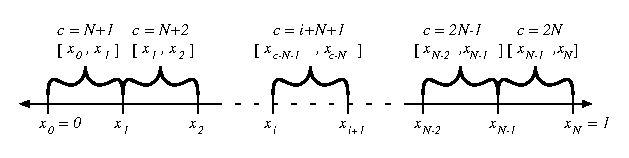
\includegraphics[width=5.50in]{figures/one-d.eps}}
%  \epsfxsize=5.50in
%  \epsfbox{figures/one-d.eps}}
 \caption{A Discretization of the Interval $[0,1]$}
 \label{fig3:oned}
\end{figure}

As illustrated in figure \ref{fig3:oned}, the discretization yields
$N+1$ interfaces which have the positions given by
\begin{equation}
x = \lbrace (i,x_i) | i \in [0, \cdots, N], x_i = i/N \rbrace.
\label{eq3:interfacex}
\end{equation}
Notice that the variable $x$ in this equation is described by a set of
ordered pairs where the first entry is the entity identifier, whereas
the second entry is the value bound to that entity.  This is a more
general abstraction of the array.  For example {\tt x[i]} is
represented abstractly as $\lbrace x_i | (i,x_i) \in x \rbrace$.

In addition, this discretization yields $N$ intervals, or cells, which
are represented by the mappings between cells and interfaces by way of
the following relationships
\begin{equation}
\begin{array}{rcl}
il & = & \lbrace (c,l) | c \in [N+1, \cdots, 2N], l = c-N-1 \rbrace,\\
ir & = & \lbrace (c,r) | c \in [N+1, \cdots, 2N], r = c-N \rbrace.\\
\end{array}
\label{eq3:cellmaps}
\end{equation}
The mappings $il$ and $ir$ provide mappings from every cell to their
left and right interfaces.  The domain of $ir$ and $il$ is $[N+1,
\cdots, 2N]$, or the cells in the discretization, while the ranges are
$\mathrm{ran}(ir) = [0, \cdots, N-1]$ and $\mathrm{ran}(il) = [1, \cdots, N]$.  This
mapping is used to conveniently describe subscripts, {\it i.e.}
$x_{c-N} = ir \rightarrow x$, where the composition operator,
$\rightarrow$, defines the application of the mapping, as in
\begin{equation}
il\rightarrow x = \lbrace (c,x_l) | (c,l) \in il, (l,x_l) \in x \rbrace.
\end{equation}
Using this notation, it is possible to conveniently describe cell
based calculations.  For example, a generic description of each cell
center is given by
\begin{equation}
\label{eq3:cellcenter}
x_c = (ir \rightarrow x + il \rightarrow x)/2.
\end{equation}
Note that the definition of $x$ provided by equation
(\ref{eq3:cellcenter}) is only applicable to cells since only cells are in
the domain of maps $ir$ and $il$; however, this does not prevent the
definition of $x$ for other entities (for example, interfaces) via
other rules.

The mappings $il$ and $ir$ are used to describe the first
step of the finite-volume discretization, where integration of
equation (\ref{eq3:diffuse}) over each cell produces the equation
\begin{equation}
\frac{d}{dt} \int_{il \rightarrow x}^{ir \rightarrow x} u dx
 =  \int_{il \rightarrow x}^{ir \rightarrow x} \nu u_{xx} dx = \nu(ir \rightarrow u_x - il \rightarrow u_x) .
\label{eq3:diffinteg}
\end{equation}

Equation (\ref{eq3:diffinteg}) is an exact equation, which can be
integrated numerically to obtain a numerical solution algorithm.
For example, when a second order mid-point rule is used to evaluate the spatial
integrations, these equations become:
\begin{equation}
\frac{d}{dt} u = \frac{\nu}{L}
\left[ {ir \rightarrow u_x - il \rightarrow u_x} \right],
\label{eq3:fvm}
\end{equation}
where 
\begin{equation}
L = \int_{il \rightarrow x}^{ir \rightarrow x} dx = ir \rightarrow x - il \rightarrow x.
\label{eq3:length}
\end{equation}

Equation (\ref{eq3:fvm}) describes the numerical method for
the spatial integrations, but it is not complete.  The gradient term,
$u_x$, located at the interfaces has not been defined as a numerical
approximation.  The most straightforward approximation for $u_x$ is a
central difference formula using the values at the cell centers at
either side of the interface.  In order to perform this calculation it
will be convenient to have a mapping from interfaces to cells similar to
the development of $il$ and $ir$.  These mappings are defined by
the relations
\begin{equation}
\begin{array}{rcl}
cl & = & \lbrace (i,l) | i \in [1, \cdots, N], l = i+N \rbrace,\\
cr & = & \lbrace (i,r) | i \in [0, \cdots, N-1], r = i+N+1 \rbrace.\\
\end{array}
\label{eq3:facemaps}
\end{equation}

Using the definitions of $cl$ and $cr$ of (\ref{eq3:facemaps}), a
numerical approximation to the gradient can be given as
\begin{equation}
  u_x = \frac{cr\rightarrow u - cl\rightarrow u}
{cr\rightarrow x_c - cl\rightarrow x_c}.
\label{eq3:ux}
\end{equation}
Notice that this equation uses the x-coordinate at the cell centers
that is computed by equation (\ref{eq3:cellcenter}).  In addition,
since this rule uses both maps $cr$ and $cl$, it only defines $u_x$ on
the intersection of the domains of $cr$ and $cl$, given by $[1, \cdots,
N-1]$.  By this reasoning, equation (\ref{eq3:ux}) only provides
gradients at the internal faces of the domain.  The gradient at the
boundary faces is provided by the boundary conditions given in
equations (\ref{eq3:diffuseb0}) and (\ref{eq3:diffuseb1}).  The
question is, how do these boundary conditions specify $u_x$ at the
boundaries without specifying $u_x$ everywhere in the domain?
Obviously additional information must be provided that constrains
the application of boundary condition gradients only to the boundary
interfaces.  A solution to this problem can be found with the
observation that the boundary interfaces have the distinction that
either $cl$ is defined or $cr$ is defined, but not both.  Using this
fact, the rules for calculating the boundary gradients can be given by
\begin{equation}
\begin{aligned}
u_x & = g(t), \mbox{constraint}\lbrace \neg \mathrm{dom}(cl) \wedge
\mathrm{dom}(cr) \rbrace, \label{eq3:brule0}\\
u & = h(t), \mbox{constraint}\lbrace \mathrm{dom}(cl)
\wedge \neg \mathrm{dom}(cr) \rbrace. %\label{eq3:brule1}
\end{aligned}
\end{equation}
Here the constraint term added to the rule indicates a constraint on
the application of the rule.  In this case it constrains the
application of the boundary conditions to the appropriate boundary faces.

At this point we have not selected the time integration method.  For
this simple example we will use the explicit first order Euler time
integration method which is expressed using the following notation:
\begin{equation}
\frac{(u^{n+1}-u^{n})}{\Delta t} = R(u^n),
\end{equation}
where
\begin{equation}
R(u) = \nu \frac{{ir \rightarrow u_x - il \rightarrow u_x} }{L}.
\label{eq3:residue}
\end{equation}
Rearranging we arrive at the following time integration scheme:
\begin{equation}
u^{n+1} = u^{n} + \Delta t R(u^n)
\label{eq3:eulerStep}
\end{equation}


At this point, the computation of $u^{n+1}$ from $u^n$ is completely
specified.  However, before any such iteration can begin, an initial
value, or $u^{n=0}$, must be given.  To be consistent with the
finite-volume formulation, the derivation of the initial conditions
begins with the integral form of equation (\ref{eq3:diffuseinitial}),
given by
\begin{equation}
\int^{ir\rightarrow x}_{il\rightarrow x} u^{n=0} dx =
\int^{ir\rightarrow x}_{il\rightarrow x} f(x) dx.
\end{equation}
Using a midpoint rule to numerically integrate this equation one
obtains the rule
\begin{equation}
u^{n=0} = f(x), \mbox{constraint}\lbrace (il,ir)\rightarrow x\rbrace.
\label{eq3:ic}
\end{equation}
For this rule, the constraint is used to indicate that although the
coordinates of the interfaces cancel in the derivation, their
existence is predicated by the integration.  In other words, the
derivation assumed a cell perspective that includes left and right
interface positions.

\section{On Problem Specification}

For an analytic solution method, equations (\ref{eq3:diffuse}) through
(\ref{eq3:diffuseb1}) are sufficient to define the problem at hand.
For numerical solution methods, additional definitions are required,
due to the fact that these are inexact methods.  For example, there
are often trade-offs between discretization and accuracy that require
additional specification.  In addition, since discretization for
complex geometries (grid generation) is not a completely automatic
process, the discretization becomes part of the problem definition for
numerical solution methods.  For the example diffusion problem already
introduced, the definition of the numerical problem consists of
spatially independent information such as the diffusion constant
$\nu$, the initial condition function $f(x)$, the numerical time step
$\Delta t$, and a representation of the discretization of space.  The
discretization of space is given by a set of positions,
(\ref{eq3:interfacex}), and the collection of mappings given in
(\ref{eq3:cellmaps}) and (\ref{eq3:facemaps}).  Table
\ref{table3:facts} summarizes these formal definitions for the example
diffusion problem.


\begin{table}[htbp]
\caption{ A Summary of Definitions for the Example Diffusion
  Problem}
\label{table3:facts}
\begin{center}
  \begin{tabular}{|l|l|}
    \hline
    fact      & meaning \\
    \hline
    $\nu$     & given diffusion constant  \\
    $f(x)$     & given initial condition  \\
    $g(t)$     & given left bc \\
    $h(t)$     & given right bc  \\
    $\Delta t$& given time-step  \\
    $x$       & $\lbrace (i,x_i) | i \in [0, \cdots, N], x_i = i/N    \rbrace$\\
    $il$      & $\lbrace (c,l)   | c \in [N+1, \cdots, 2N], l = c-N-1 \rbrace$\\
    $ir$      & $\lbrace (c,r)   | c \in [N+1, \cdots, 2N], r = c-N   \rbrace$\\
    $cl$      & $\lbrace (i,l)   | i \in [1, \cdots, N], l = i+N      \rbrace$\\
    $cr$      & $\lbrace (i,r)   | i \in [0, \cdots, N-1], r = i+N+1  \rbrace$\\
    \hline
  \end{tabular}
\end{center}
\end{table}



\section{On Specification of Process}

Given the definition of the problem, the process of solving the
problem is dictated by a prescribed set of transformations.  For
example, consider equation (\ref{eq3:cellcenter}) as an example of a
transformation that transforms $x$ located at $il$ and $ir$ into a
cell $x_c$.  To simplify discussions of the structure of the
calculations, the transformation rules are represented by a rule
signature that is denoted by a list of targets of the transformation
delineated from the sources of the transformation by the left arrow
symbol, '$\leftarrow$'.  Thus the cell center position calculation is
represented by the rule signature $x \leftarrow (ir,il)\rightarrow x$.
This rule signature represents the augmentation of the set of ordered
pairs defined in equation (\ref{eq3:interfacex}) with the additional
set given as
\begin{equation}
x_c \leftarrow\lbrace (c, x_c) |  x_c = (x_l + x_r)/2,
                               (l,x_l) \in x, (r,x_r) \in x, 
                               (c,l) \in il, (c,r) \in ir \rbrace.
\end{equation}
For the moment, the augmentation of $x$ with this set can be
considered as a set union operation, with the caveat that it will
become more complex once issues of specification consistency are
considered.  Given this notation, the specification of the
finite-volume scheme derived in this section can be summarized by
eight rules given in table \ref{table3:rules}.

\begin{table}[htbp]
\caption{ A Summary of Rules Describing the Solution of the Example
    Diffusion Problem.}
\label{table3:rules}
\begin{center}
  \begin{tabular}{|l|l|l|}
    \hline
    Rule  & Rule Signature & Equation\\
    \hline
    Rule 1 & $x_c \leftarrow (ir,il)\rightarrow x $ &
    (\ref{eq3:cellcenter})\\
    Rule 2 & $ L \leftarrow (ir,il)\rightarrow x $ &
    (\ref{eq3:length})\\
    Rule 3 & $u_x \leftarrow (cr,cl)\rightarrow(u,x_c)$ &
    (\ref{eq3:ux})\\
    Rule 4 & $u_x \leftarrow  h, t, \mbox{constraint}\lbrace 
    \mathrm{dom}(cl) \wedge \neg \mathrm{dom}(cr) \rbrace$ &
    (\ref{eq3:brule0})\\
    Rule 5 & $u_x \leftarrow  g, t, \mbox{constraint}\lbrace 
    \mathrm{dom}(cr) \wedge \neg \mathrm{dom}(cl) \rbrace$ &
    (\ref{eq3:brule0})\\
    Rule 6 & $R\leftarrow \nu,L,(ir,il)\rightarrow u_x$ & (\ref{eq3:residue})\\
    Rule 7 & $u^{n+1} \leftarrow u^n, R^n, \Delta t$ & (\ref{eq3:eulerStep})\\
    Rule 8 & $u^{n=0} \leftarrow f,x_c,\mbox{constraint}\lbrace(il,ir)\rightarrow
    x\rbrace $ &
    (\ref{eq3:ic})\\
    \hline
  \end{tabular}
\end{center}
\end{table}

\section{On Interpreting the Problem Specification}

The eight rules described in the preceding section form the basis of
creating a {\it Loci} program.  Before we consider how to do this, lets
first consider how the facts given in table \ref{table3:facts} and the
computational elements described in table \ref{table3:rules} can be
composed to create a time dependent simulation.  Note, that the final
values of interest are the values for $u^n, n=0,1, \cdots$.  It is
clear to see that rules 7 and 8 describe how to accomplish this
computation.  However, more information is needed to complete the
operation, specifically note that we need the residual $R$ evaluated
at iteration level $n$, denoted by $R^n$.  However, also note that the
residual rule given by rule 6 does not have a time notation (no
superscript $n$).  This rule is said to be described at stationary
time, that is the relationship is established as an invariant to
iteration.  That is, R is defined as the same relationship among
variables regardless of iteration identifier.  In this case, we know
that we will need to compute $R$ for every time-step because it is a
function of $u$ which itself is dependent on the iteration.  Usually
when converting a paper description of an algorithm a program
implementation we need to make these determinations.  In {\it Loci}, this is
automatically performed by time promotion deductions.  That is, {\it Loci}
will automatically determine that the residual and gradients of $u$
will need to be recomputed each time-step, while $x_c$ and $L$ will
not.  To accomplish this {\it Loci} will invoke either rule promotions or
variable promotions, that is that if we have a rule
$x_c\leftarrow(ir,il)\rightarrow x$ then {\it Loci} may either promote the
rule to the iteration (e.g $x_c^n\leftarrow(ir^n,il^n)\rightarrow
x^n$, or promote the variable to the iteration (e.g. $x_c^n\leftarrow
x_c$), as needed to satisfy the computation.  As a policy, {\it Loci} only
schedules computations at an iteration as required, all other
computations are performed once and reused through iterations using
variable promotion.

\section{Creating the Fact Database}

Before we begin performing computations we have to describe how to
express the information in table \ref{table3:facts} as a {\it Loci} fact
database ({\tt fact\_db}).  The code we are about to describe is
included in the {\tt 1D-Diffusion} directory in the {\it Loci} tutorial.
The facts described in this table are essentially the result of a one
dimensional grid generation process that is handled by the {\tt
  generate\_grid} function as described below:
\begin{verbatim}
// Generate a 1d grid over the number line from [0,1] consiting of N segments
// The resulting grid is installed in the fact_db facts 
void generate_grid(fact_db &facts, int N) {
\end{verbatim}
The first step to generating this discretization of the interval
$[0,1]$ is to allocate space for the nodes and cells that will
comprise the final grid.  We ask the fact database to generate unique
entity numbers for these entities using the {\tt get\_allocation() }
method:
\begin{verbatim}
  // Allocate the nodes and cells of the grid
  entitySet nodes = facts.get_allocation(N+1) ;
  entitySet cells = facts.get_allocation(N) ;
\end{verbatim}
Now that we have these allocations we can first create the fact
``x''.  This fact use the {\tt store} container as it is an
association of floating point values with entities.  This container is
first allocated over the prescribed entities.  The values are assigned
by giving the lowest numbered entity the value of $x=0$, and then
adding a delta x to subsequent values.  The resulting values are then
placed in the fact database using the {\tt create\_fact} method, as
shown below:
\begin{verbatim}
  // setup x coordinates for nodes
  store<float> x ;
  x.allocate(nodes) ;
  float dx = 1./float(N) ; // Uniform delta x
  entitySet::const_iterator ni ;
  float xtmp = 0 ;
  // iterate over nodes and assign positions by adding dx to
  // preceeding x value
  for(ni=nodes.begin();ni!=nodes.end();++ni) {
    x[*ni] = xtmp ;
    xtmp += dx ;
  }
  // Add node positions to facts
  facts.create_fact("x",x) ;
\end{verbatim}

Now we need to develop the connectivity relations between cells and
nodes as described by {\tt cl} (cell left), {\tt cr} (cell right),
{\tt il} (interface left), and {\tt ir} (interface right).  Note that
while all cells will have a value for {\tt il} and {\tt ir}, only the
interior nodes will simultaneously have values for {\tt cl} and {\tt
  cr}.  To compute the nodes that will be used for these maps, we use
the shifting operator of the entity set which adds or subtracts values
from all entity identifiers, as in:
\begin{verbatim}
  // Find the nodes that are on the left and right side of cells
  // by shifting the allocated numberings to the left or right by one
  entitySet left_nodes = (nodes >> 1) & nodes ;
  entitySet right_nodes = (nodes << 1) & nodes ;
\end{verbatim}
We now have the sets needed to allocate these containers.  Note that
since we are describing a relationship between various entities, the
container that we use is a {\tt Map}.  A Map can be thought of as a
{\tt store} that contains entity identifiers instead of values.  The
allocation is performed as follows:
\begin{verbatim}
  // Allocate maps for the left cell and right cell of a node
  Map cl,cr,il,ir ;
  cl.allocate(left_nodes) ;
  cr.allocate(right_nodes) ;
  il.allocate(cells) ;
  ir.allocate(cells) ;
\end{verbatim}
Now we are able to create these {\tt Map}s.  We use a technique of
finding a correspondence between left nodes and cells or right nodes
and cells to establish this relationship.  In addition, we build both
{\tt cl} and {\tt ir} at the same time recognizing that one map is
simply the transpose of the other as illustrated below:
\begin{verbatim}

  entitySet::const_iterator ci ;
  // Assign left nodes to cells in consecutive order
  ci = cells.begin() ;
  for(ni=left_nodes.begin();ni!=left_nodes.end();++ni,++ci) {
    cl[*ni] = *ci ;
    ir[*ci] = *ni ;
  }
  // Assign right nodes to cells in consecutive order
  ci = cells.begin() ;
  for(ni=right_nodes.begin();ni!=right_nodes.end();++ni,++ci) {
    cr[*ni] = *ci ;
    il[*ci] = *ni ;
  }
\end{verbatim}
We now install these relations in the fact database:
\begin{verbatim}
  facts.create_fact("cl",cl) ;
  facts.create_fact("cr",cr) ;
  facts.create_fact("il",il) ;
  facts.create_fact("ir",ir) ;
\end{verbatim}
Now we must compute the entities that are on the boundaries.  We do
this by examining the domain (entities for which a container has a
definition) of the {\tt cl} and {\tt cr} maps, similar to the previous
specifications.  There are two boundaries in this one dimensional
problem, the left boundary and the right boundary.  They are
represented by {\tt constraint} containers which are special data
types used in {\it Loci} to give sets of entities special attributes.  The
boundary condition constraints are specified below:
\begin{verbatim}
  // Identify boundary conditions
  constraint left_boundary ;
  constraint right_boundary ;
  *right_boundary = cl.domain() - cr.domain() ;
  *left_boundary = cr.domain() - cl.domain() ;

  facts.create_fact("left_boundary",left_boundary) ;
  facts.create_fact("right_boundary",right_boundary) ;
\end{verbatim}
Finally, for some computations it is useful to identify the geometric
cells in the problem (for example if ghost cells were employed.)  Here
we can easily create such an identification using a constraint as in:
\begin{verbatim}
  constraint geom_cells ;
  *geom_cells = cells ;
  facts.create_fact("geom_cells",geom_cells) ;
\end{verbatim}

Now we have created a {\it Loci} implementation of the facts described in
table \ref{table3:facts}.  To complete the {\it Loci} implementation we will
need to describe the rules as well.  This is discussed next.

\section{Creating the rule database}

To capture what is specified in the table \ref{table3:rules} we will
create a database of rules.  To simplify this process we use the {\it
  Loci} preprocessor that will convert rule specifications into
standard C++ code.  A program that has a {\tt .loci} postfix will
automatically be compiled with the {\it Loci} preprocessor if you use
one of the provided example makefiles.  Any valid C++ source file is
also a valid {\it Loci} preprocessor file, that is we are free to mix
standard C++ code and {\it Loci} specific directives in this file.
The {\it Loci} preprocessor becomes activated through the use of the
``{\tt \$}'' symbol as will be described in the following paragraphs.

In the beginning you will want to tell the {\it Loci} preprocessor
what the types of the {\it Loci} variables that you will be working
with.  For example, the {\it Loci} preprocessor will need to know what
the types of the facts that were created earlier to describe the
one-dimensional mesh.  We can describe the types to the preprocessor
using the {\tt \$type} keyword.  This first argument after this
keyword is the variable name, while the second argument is the type.
The statement ends with a semicolon.  For example, the type
definitions for the initial fact database are given by:
\begin{verbatim}
// Setup Types for initial facts
$type il Map ; // interface left
$type ir Map ; // interface right
$type cl Map ; // cell left
$type cr Map ; // cell right
$type x store<float> ; // node positions
\end{verbatim}

Generally we would like to share types between separate files to
simplify compilation and source code management.  It is possible to do
this with the {\it Loci} preprocessor.  For example, the above definition
can be put into a header file, say the file {\tt "mesh.lh"} and then
included into the {\it Loci} program using the keyword {\tt \$include}.
NOTE: this must be {\tt \$include} not the C preprocessor directive
{\tt \#include}!  For example, to include the above type information
file use the line:
\begin{verbatim}
$include "mesh.lh"
\end{verbatim}

\subsection{Specifying User Tunable Inputs}
Before we begin specifying the {\it Loci} rules as described in table
\ref{table3:rules}, lets discuss feature of {\it Loci} that allow the user
to easily change some of the facts used to describe the simulation.
In this case, the user may want to change the viscosity, the number of
cells in the discretization, or the number of time-steps to simulate.
All of these parameters can be given default values using special {\it Loci}
rules, and then the user can change these default values by providing
a special ``vars'' file.  For example, we can specify the default
values for these parameters with the following lines of code:
\newpage
\begin{verbatim}
// Input parameters
$type N param<int> ;              // How many nodes
$type nu param<float> ;           // diffusion coefficient

$rule default(N) {
  $N=50 ;
}

$rule default(nu) {
  $nu = 1.0 ;
}
\end{verbatim}

In these lines of code we can see our first {\it Loci} rules.  The rules are
preceded with {\tt \$type} specifiers so that {\it Loci} will know the types
of the variables.  Then the {\tt \$rule} specifier tells the {\it Loci}
preprocessor that a rule is about to be defined.  Immediately after
the {\tt \$rule} specifier is the rule type that specifies the type of
the rule.  The rule signature is provided in the parenthesized region,
while the braces enclose the code actually executed when the rule is
required.  The {\tt default} rule type is specifically to provide a
mechanism for users to change a given value in the fact database, but
also to provide a default value if the user does not specify one.
Note the use of the ``{\tt \$} '' to identify the {\it Loci} variables in
the computational part that is enclosed in braces.  We also note that
we provide the {\tt optional} rule type to specify values that the
user can provide, but for which no default value will be provided if
the user provides no value.  In this case, the facts will simply not
contain this attribute. 

To utilize these {\tt default} and {\tt optional} rule types, the user
must specifically read in values from a user provided file.  For
example, we read in the user provided values from a file called {\tt
  heat.vars} in the file {\tt main.cc} with the following code:

\begin{verbatim}
  string varsFile = "heat.vars" ;
  facts.read_vars(varsFile,rdb) ;
\end{verbatim}

The user provided vars file consists of a braces delimited list of
variable assignments.  For example, a typical {\tt heat.vars} file
might look something like:
\begin{verbatim}
{
N: 10
nu: 10.0
}
\end{verbatim}

\subsection{Basic Rule Specification}
Now we can begin with the implementation of the rules described in
table \ref{table3:rules} in {\it Loci}.  The first of these rules is the
computation of the cell center, denoted by the variable {\tt xc} which
is represented in {\it Loci} by the following code:
\newpage
\begin{verbatim}
// Rule 1: compute the cell center from node positions
$rule pointwise(xc<-(il,ir)->x) {
  $xc = .5*($il->$x + $ir->$x) ;
}
\end{verbatim}
In this specification, the {\tt \$rule} directive tells the loci
preprocessor that we are about to describe a {\it Loci} rule.  The
keyword {\tt pointwise} that follows indicates that the rule
represents a point by point computation.  The parenthesis that follow
describe the rule signature which documents what the rule will use for
inputs and outputs.  Note that the comma in the rule signature binds
most tightly, so we use parenthesis to group items.  For example,
{\tt(il,ir)->x} means the same thing as {\tt il->x,ir->x}.  Similarly,
{\tt il->(x,y)} would mean {\tt il->x} and {\tt il->y}, whereas {\tt
  il->x,y} would mean {\tt il->x} and {\tt y}.  Note, when several
variables are listed on both the sides of the ``{\tt ->}'' operator,
then all combinations are implied.  Thus {\tt (il,ir)->(x,y)} is
equivalent to {\tt il->x} and {\tt ir->x} and {\tt il->y} and {\tt
  ir->y}.  The code that follows the signature is the actual
implementation of equation (\ref{eq3:cellcenter}) where the ``{\tt
  \$}'' is used to identify the use of {\it Loci} variables.  NOTE: It
is important that the rule signature match the implementation: if {\tt
  \$il->\$x} is in the implementation then {\tt il->x} needs to be in
the rule signature.  If not, then {\it Loci} may schedule the rule
incorrectly.

\subsection{Boundary Conditions and Constraints}

Rule 3 provides a method for computing interface gradients.  However,
this rule only provides values for the internal interfaces as these
are the only interfaces that have both {\tt cl} and {\tt cr}
attributes.  Boundary conditions are used to define {\tt ux} at the
left and right boundaries. For example, at the left boundary $u_x =
h(t)$.   If we simply defined a rule to define {\tt ux} in this way,
how do we limit the specification to only apply to the left boundary?
To do this we use a rule constraint.  The rule constraint is a set of
entities that constrain the rule application.  A constraint applied to
the rule makes two assertions: 1) the rule can only be applied for
entities in found in the constraint set, and 2) all inputs to the rule
must be available for the entire set of entities found in the
constraint. Thus, we can use the {\tt left\_boundary} constraint that
was placed in the fact database to apply this boundary condition as
illustrated in the following code:

\begin{verbatim}
// Neuman boundary condition at left boundary, ux = h(t)
$rule pointwise(ux<-h), constraint(left_boundary) {
  $ux = $h ;
}
\end{verbatim}

\subsection{Specifying Iterating Algorithms}
The implementation of rules 2-6 follow a similar procedure as rule 1,
and can be found in the tutorial under the file ``{\tt heat.loci}''.
The time-stepping rules 7 and 8 require a bit more discussion.  First
we need to discuss how we represent the superscripts in this rule
notation.  For example, how is $u^n$ represented in {\it Loci} code?  The
superscript is represented in a brace delimited region that follows the
variable name, so that $u^n$ becomes {\tt u\{n\}} in a {\it Loci} rule
signature and {\tt \$u\{n\}} in the implementation. Also note that the
type specifications don't include the superscript, therefore the type
statement for this variable will be:
\begin{verbatim}
$type u store<float> ; // Solution variable
\end{verbatim}

Now we can specify rules 7 and 8 in a straightforward manner as follows:
\begin{verbatim}
// Rule 7: initialization of iteration (build rule)
$rule pointwise(u{n=0}<-xc) {
  $u{n=0} = f($xc) ;
}

// Rule 8: time advance using explicit Euler time integration algorithm
$rule pointwise(u{n+1}<-u{n},dt{n},R{n}) {
  $u{n+1} = $u{n}+$dt{n}*$R{n} ;
}
\end{verbatim}

Note that the above to rules play different roles in describing the
iteration.  Rule 7 is called a ``build'' rule in {\it Loci}.  It describes
how to build the initial values of an iteration.  It is distinguished
by having an output at with a time specification that includes the
``='' operator.  Rule 7 is called an ``advance'' rule in {\it Loci}.  The
advance rule describes how to advance a variable to the next
iteration.  It is characterized by having an output that is at an
advanced time level from its inputs.  These two rules tell {\it Loci} how to
iterate the variable {\tt u} forward in time, but does not describe
how, or when, to end the iteration.  For this we need a collapse rule
which is a rule that tells {\it Loci} how to compute a value that results
from the iteration.  For example, we might have a collapse rule that
computes a variable called ``{\tt solution}'' that represents the
solution of the time integration problem.  Such a rule would be
represented as:
\begin{verbatim}
$rule pointwise(solution<-u{n}),conditional(simulation_finished{n}) {
  $solution = $u{n} ;
}
\end{verbatim}
Notice that this rule has an additional ``{\tt conditional}'' clause.
This clause is used to tell {\it Loci} when it is OK to terminate or
``collapse'' the iteration.  This termination condition will be
provided by another rule as described next.  For the moment we will
use the criterion that when the iteration variable {\tt n} reaches a
predetermined value, the loop will terminate.  This is accomplished
with the following code:

\begin{verbatim}
$type max_iteration param<int> ;
$type simulation_finished param<bool> ;

// Condition that determines when iteration is complete
$rule singleton(simulation_finished<-$n,max_iteration) {
   $simulation_finished = ($$n >= $max_iteration) ;
}
\end{verbatim}

First notice that the type of {\tt simulation\_finished} is a bool
parameter.  This is a single boolean value shared by all of the
iterating entities.  The loop will terminate when this value evaluates
to {\it true}.  Also notice that this rule is a {\tt singleton} rule.
This means that the rule is computing a single value.  Singleton rules
are used to compute parameters from other parameters, and thus apply
to single values rather than collections arrayed over entities.
Finally, notice that we can access the value of the iterating
superscript by using the ``{\tt \$n}'' variable name.  This is a
special variable (always typed as an integer parameter) that contains
the current iteration number.  Also, notice that when using this
variable in the implementation, two ``{\tt \$}'' symbols appear.  The
purpose of this rule should be clear at this point: when {\tt \$n} is
equal to {\tt max\_iteration} then {\tt simulation\_finished} is
true, otherwise it is false.  Thus this specifies when {\it Loci} should
terminate the iteration.

\subsection{Next Step: Global Reductions}

The above specification is nearly complete.  However we have left out
one important detail and that is the specification of the time-step,
$\Delta t$.  How do we arrive at this time-step size?  One approach
would be to have the user specify this parameter by providing a
{\tt default} rule.  This would allow the user to input a specific
time-step.  However, since the explicit Euler time-stepping algorithm
has a stability bound, it might be better if the solver computed a
stable time-step.  The stability limit for this algorithm is given by
the equation:
\begin{equation}
\Delta t = \frac{1}{2}\frac{L^2}{\nu}.
\end{equation}
However, since it is possible for the mesh to be non-uniform in our
formulation, we would like to find out what is the smallest possible
time-step by applying this equation to all possible cells.  We can
accomplish this operation by using a global reduction.  For a global
reduction, the output of the rule is a parameter, indicating that
there will be a single value shared by many entities.  Reductions in
{\it Loci} are specified using two different rule types: {\tt unit} and {\tt
  apply}.  A reduction is always defined with respect to some operator
that 1) has an identity, 2) is associative, and 3) is commutative.
In this example we will use the minimum operator that an identity (the
largest possible number) and is associative and commutative.  The
computation of the global stable time-step is given by the following
{\it Loci} code:
\begin{verbatim}
$type dt param<int> ; // simulation timestep

$rule unit(dt), constraint(UNIVERSE) {
   $dt = std::numeric_limits<float>::max() ; // largest allowble timestep
}

$rule apply(dt<-L,nu)[Loci::Minimum] {
    float local_dt = $L*$L/(2.*$nu) ;  // Stable timestep
    join($dt,local_dt) ; // Set dt = min(dt,local_dt)
}
\end{verbatim}

Here we see the unit rule being applied to compute the identity of the
operator.  In this specific case we use the C++ standard to query the
maximum floating point value to assign to {\tt dt}. Notice that we
provide a constraint of {\tt UNIVERSE} which indicates that {\tt dt}
will be associated with all entities in the simulation.  The rule that
follows is the apply rule that specifies that the {\tt Loci::Minimum}
operator will be used.  {\it Loci} provides the following operators: {\tt
  Loci::Summation}, {\tt Loci::Product}, {\tt Loci::Maximum}, and {\tt
  Loci::Minimum}.  Other operations can be defined by the user as will
be described in later sections.  Here the apply rule uses the {\tt
  join} operator to combine the local stable time-steps with the
global time-step.  The first argument to the join operator is the
variable that is being reduced, while the second argument is the
variable that is being combined.  

Note, there are some important cautions that should be mentioned
here.  First, it is important that the unit rule assigns the identity
value because it is possible that this rule may be computed and
combined multiple times (particularly in the parallel), therefore it
is not OK, for example, to have the unit rule assign a partial sum
expecting that the value will only be added once.  Second, it can be
deceptively easy to violate the associative and commutative properties
of the operator.  For example, consider the following {\it Loci} code:
\begin{verbatim}
$rule apply(sum<-terms)[Loci::Summation] {
    if($sum < 1) // Error!  Result depends on order terms are summed!
      join($sum,$terms) ; 
}
\end{verbatim}
Note, it is not the if statement that is wrong, but rather the
conditional on the partially summed result.  For example, the
following code is OK:
\begin{verbatim}
$rule apply(sum<-terms)[Loci::Summation] {
    if($terms < 1) // OK, result is independent of summing order
      join($sum,$terms) ; 
}
\end{verbatim}

\subsection{The {\it Loci} Generated Schedule}

The one dimensional heat solver that is provided with the tutorial can
be used to see how {\it Loci} will create a program from the rules we have
described to create a heat solver. An execution schedule is generated
by {\it Loci} automatically when the user issues a {\tt
  Loci::makeQuery()} function call.  The last argument of this
function call is the name of the variable that you desire.  By
default, we usually query for a variable called ``solution'' which
represents the generic solution of a problem and plays a similar role
to {\tt main} in C programs.  Since the collapse rule of our Euler
time-step algorithm generates the variable ``solution'', a query for
this variable will produce a schedule that solves the time-dependent
heat equation.  By default, this schedule is not provided to the users
of {\it Loci}, but {\it Loci} can be instructed to print this schedule
in human understandable form.  For example, to see the schedule
generated by the heat solver, you can execute:
\begin{verbatim}
./heat --scheduleoutput --nochomp
\end{verbatim}
The {\tt --scheduleoutput} instructs {\it Loci} to write out the
generated schedule into a file called ``.schedule'' (on a single
processor).  The {\tt --nochomp} instructs {\it Loci} to not perform
the chomping optimization on the program.  This will make the schedule
a little bit easier to read and understand.

Before we look at the entire program, lets first consider what happens
if we query for a variable that is easier to compute, for example the
time-step control, {\tt dt}.  The heat program contains code for the
user to specify a query different from ``solution'' by using the {\tt
  -q} flag.  Thus we can query for the stable time-step using the
command:
\begin{verbatim}
./heat --scheduleoutput --nochomp -q dt
\end{verbatim}

In addition to computing the stable time-step, this command generates a
file called {\tt .schedule} that contains the execution schedule:
\begin{verbatim}
dt<-CONSTRAINT(UNIVERSE) over sequence ([0,20])
L<-(il,ir)->x over sequence ([11,20])
dt<-L,nu over sequence ([11,20])
\end{verbatim}

Here we see first that the unit rule for the dt computation is
called.  The sequence is the set of entities that requested {\tt dt}.
Then {\tt L} is computed because this will be needed by the {\tt dt}
apply rule that follows.  Notice, both of these rules execute over the
sequence {\tt [11,20]} which are the entity identifiers for the
cells in the problem.  Once this is computed, the {\tt dt} is
successfully computed and the execution schedule terminates.  Now lets
see what happens when we query for solution:

\begin{verbatim}
dt<-CONSTRAINT(UNIVERSE) over sequence ([0,20])
ub<-g,CONSTRAINT(right_boundary) over sequence ([10,10])
xc<-(il,ir)->x over sequence ([11,20])
L<-(il,ir)->x over sequence ([11,20])
dt<-L,nu over sequence ([11,20])
promote:cr{n}<-cr
promote:left_boundary{n}<-left_boundary
promote:h{n}<-h
promote:ub{n}<-ub
promote:cl{n}<-cl
promote:xc{n}<-xc
promote:x{n}<-x
promote:max_iteration{n}<-max_iteration
promote:L{n}<-L
promote:ir{n}<-ir
promote:il{n}<-il
promote:nu{n}<-nu
promote:dt{n}<-dt
ux{n}<-h{n},CONSTRAINT(left_boundary{n}) over sequence ([0,0])
u{n=0}<-xc over sequence ([11,20])
generalize:u{n}<-u{n=0}
Iteration Loop{n} {
    simulation_finished{n}<-$n{n},max_iteration{n} over sequence ([11,20])
    if(simulation_finished{n}) {
      solution<-u{n},CONDITIONAL(simulation_finished{n}) over sequence ([11,20])
    } // if(simulation_finished{n})

    -------------- Exit of Loop{n}
    if(simulation_finished{n}) break ;

    ux{n}<-(cl{n},cr{n})->(u{n},xc{n}) over sequence ([1,9])
    ux{n}<-cl{n}->(u{n},xc{n}),ub{n},x{n} over sequence ([10,10])
    R{n}<-(il{n},ir{n})->ux{n},L{n},nu{n} over sequence ([11,20])
    u{n+1}<-R{n},dt{n},u{n} over sequence ([11,20])
} // {n}
\end{verbatim}

While this schedule is similar to the previous schedule, we observe
many new features that weren't present in the previous example.  First
we see that in the beginning several variables are computed that will
be used during the time-stepping portion of the algorithm.  This is
followed by a sequence of variable promotion operations indicated by
lines such as:
\begin{verbatim}
promote:cr{n}<-cr
\end{verbatim}
This line indicates that the variable {\tt cr} will be used unchanged
during the {\tt n} iteration.  In essence it is basically indicating
that {\tt cr} and {\tt cr\{n\}} are the same variable.  This will
allow rules that have been promoted to the time-stepping iteration to
access these variables.  We then notice that the initial conditions
are then computed followed by a variable generalization given by:
\begin{verbatim}
generalize:u{n}<-u{n=0}
\end{verbatim}
This indicates that for the first iteration {\tt u\{n\}} is the same
as {\tt u\{n=0\}}.  Note that after the first iteration, {\it Loci}
sets {\tt u\{n\}} to the previous iteration value that was computed
for {\tt u\{n+1\}}.  

After the generalize rule, we begin the iteration loop.  The first
operation performed is to compute the condition for collapsing
(terminating) the loop.  If this is true, the schedule executes the
collapsing code and then exits the loop.  Otherwise, the loop
continues to compute the next iteration value, {\tt u\{n+1\}} using
the provided rules.  First the gradients are computed (with the
exception of the Neumann BC that was computed in advance).  Then the
residual is computed using these gradients.  And finally, the Euler
time integration rule is used to advance the variable {\tt u} to the
next iteration.  Once this is complete, {\it Loci} advances $n$ and
begins again.

Notice that everything Loci needed to form this schedule could be
inferred from the rules that were provided in the previous sections.
Looking at the schedule generated by Loci can be helpful in learning
how to use {\it Loci}.  Experiment with changing how rules are
implemented, what they input, for example, and examine how this
changes the schedule.  For example, what happens if the stable
time-step computation input the variable {\tt u}?  What changes would
{\it Loci} need to make to the schedule?

\subsection{Local Reductions: An Alternative}

The fact database described in this example included two sets of
maps.  One set of maps provided an association from cells to
interfaces ({\tt il,ir}), and another provided an association from
interfaces to cells ({\tt cl,cr}).  However, these maps are
intrinsically related to one another in that {\tt il} is the transpose
of {\tt cr} and {\tt ir} is the transpose of {\tt cr}.  Since these
maps represent a storage overhead, it is reasonable to ask if they are
both necessary.  In fact, we can eliminate one pair of maps if we
reorganize some of our computations so that they shift from being cell
centric to being interface centric.  Note, that this represents a
common trade-off found in unstructured solver algorithms, and {\it Loci}
provides techniques that allows us to develop algorithms that can
reduce the amount of connectivity storage required.  

For example, consider the computation of the cell centers described
by the rule:
\begin{verbatim}
$rule pointwise(xc<-(il,ir)->x) { $xc = .5*($il->$x + $ir->$x) ; }
\end{verbatim}

This rule is cell centric: the context of the rule (where computations
occur) is cells, as cells are the entities that have attributes {\tt
  il} and {\tt ir}.  Can we transform this rule so that it uses the
face centric maps {\tt cl} and {\tt cr}?  Yes, we can.  But the
resulting computation is somewhat less straightforward.  Essentially
the computation is transformed whereby we visit all of the interfaces
in the line and each interface will add half of its position to each
side.  When all interfaces add their parts, then the final total will
be the cell center.  This computation is similar to the global
reduction described earlier with one important difference: this
computation results in many cell centers, not just one.  This
many-to-many reduction process is called a local reduction.  A local
reduction is described in the same way as a global reduction in {\it Loci},
the only difference is that the result of the local reduction is a
store rather than a parameter.  Thus, we use a unit/apply combination
to describe the computation much like the previous example.  Here is
an example of three rules that can replace the cell center computation
using {\tt cl} and {\tt cr} maps:
\begin{verbatim}
$rule unit(xc), constraint(geom_cells) {  $xc = 0 ; }
$rule apply(cl->xc <- x)[Loci::Summation] {  join($cl->$xc,.5*$x) ; }
$rule apply(cr->xc <- x)[Loci::Summation] {  join($cr->$xc,.5*$x) ; }
\end{verbatim}
First note that we have a unit rule that assigns the value of the cell
center to the identity of summation (zero).  Also note that the rule
is constrained to exist only for geometric cells (we put this
constraint {\tt geom\_cells} in the fact database, as described
earlier).  This constraint keeps this rule from defining values for
entities that are not cells.  Now to compute the cell center we look
at each interface and add half its position to both the left and right
sides.  These three rules are equivalent to Rule 1, but use the maps
{\tt cl} and {\tt cr} instead.  Note that the map appears in the
output of the rule rather than the input, and this is essentially how
the map becomes transposed.  In fact, as a rule of thumb, usually
pointwise rules have mappings in the inputs, while apply rules have
mappings in their outputs for exactly this reason.  Applying this
technique to other rules that use {\tt il} and {\tt ir} it is possible
to completely eliminate the need for these maps.

{\it Note: it would be tempting to combine these two rules
into one adding to both the left and right sides at the same time.
However, the boundary faces would be left out in this case, since they
don't have both a left and right side.}


\subsection{Getting Sophisticated: Parametric Rules}

When developing {\it Loci} rules, one quickly will notice patterns that are
repeated in many different rules.  In such cases it would be useful to
define a family of rules that can be called upon to act on different
variables.  For example, it would be useful to define a gradient
operator that could apply to different variables, then rather than
have variable {\tt ux} and an associated rule to compute this specific
gradient, it would be useful to have a way of specifying {\tt grad(u)}
instead.  We can do this using parametric rules.  For this one
dimensional heat equation, there are several cases where it would be
useful to have a parametric rules to capture these common structures.
One example is the integration of fluxes that results in a difference
between interfaces.  It would be useful to have a cell integral
function to perform this common operation.  In addition, specifying
this as a parametric rule will simplify the process of converting to
using the {\tt cl} and {\tt cr} maps.  

Parametric rules are defined when parametric variables are used in
their outputs.  A parametric variable is one that has parameters as
defined by a parenthesized list of substitution keys.  Thus, for
example, if we want to create a cell integration of some variable, we
can provide that using the parametric variable {\tt cellIntegrate(X)}.
How {\it Loci} interprets the parametric variables depends on where the
variable occurs in the rule signature.  If the parametric variable is
in the output of a rule, then the rule is parametric and describes a
family of rules that can be obtained by performing substitutions of
the keys listed in the argument list.  However, if the parametric
variable is in the input, then it becomes a request for an
instantiation of a specific version of the parametric rule that is
obtained by substituting the provided arguments for the substitution
keys given in the parametric rules.  This may seem somewhat confusing,
but it is actually very straightforward once you see it in action.

For example, suppose that we wished to create rule that could
integrate from the bounding interfaces of a cell as is obtained from
flux integrations used in the residual equation.  We could create a
parametric rule to describe an arbitrary integration such as the
following code segment:

\begin{verbatim}
$type cellIntegrate(X) store<float> ;
$type X store<float> ;

$rule pointwise(cellIntegrate(X)<-(il,ir)->X) {
   $cellIntegrate(X) = $ir->$X - $il->$X ;
}
\end{verbatim}

What this rule represents is that for some arbitrary variable {\tt X},
{\tt cellIntegrate} can be computed for a given variable, say {\tt R},
by substituting {\tt X} for {\tt R} in the above rule.  Thus once we
have the rule above we can compute the residual with the following rule:

\begin{verbatim}
// The 1d diffusion residue
$rule pointwise(R<-nu,cellIntegrate(ux),L) { $R = $nu*$cellIntegrate(ux)/$L ;}
\end{verbatim}

Note, that once we have defined this integral, we can use it in other
places which could be described in terms of this form of definite
integral.  For example the length of a cell can actually be
represented as an integral of this form, thus we can also use the
parametric rule to compute {\tt L} as follows:

\begin{verbatim}
// We find the length of an interval by integrating the position x
$rule pointwise(L<-cellIntegrate(x)) { $L = $cellIntegrate(x) ; }
\end{verbatim}

Parametric rules behave somewhat like subroutines and share many of
the same advantages.  One advantage is that because many related
functions share the same implementation, it is possible to replace on
method of computation with another that is transparent to other parts
of the computations.  In the same way, the use of the {\tt
  cellIntegrate} parametric rule will allow us to change fewer parts
of the program to transform from a cell centric integration as
described earlier, to a face centric integration that uses local
reductions.  Note that parametric rules are compatible with all types
for rule specifications and can be used with unit and apply rules.
Thus, we can replace the earlier cellIntegrate formulation with the
following set of rules to eliminate the use of the {\tt il} and {\tt
  ir} mappings, as is demonstrated with the following code:

\begin{verbatim}

// A general function for integrating over a cell boundary
$rule unit(cellIntegrate(X)),constraint(geom_cells) {
  $cellIntegrate(X) = 0 ;
}
$rule apply(cl->cellIntegrate(X)<-X)[Loci::Summation] {
  join($cl->$cellIntegrate(X),$X) ;
}
$rule apply(cr->cellIntegrate(X)<-X)[Loci::Summation] {
  join($cr->$cellIntegrate(X),-$X) ;
}
\end{verbatim}

\subsection{Iterations and Parametric Rules}

It is reasonable to ask if we can build iterative algorithms using
parametric rules.  The answer is: yes we can.  For example, if we could
build the explicit Euler time integration using parametric rules, then
we could employ this time integration method with other residual
equations to build various different types of solvers.  Here, let us
demonstrate how to build a parametric explicit Euler solver to show
how it is done.  First we need to define what parameters are needed to
define the integration method.  We select two parameters, the first is
the function to be integrated, and the second is the variable of
integration.  With such a specification we would only need to query
for {\tt EulerIntegrate(R,u)} to perform the integration of the
diffusion equation described earlier.  Now lets see how we accomplish
this goal.  First we will need to define the types of the variables we
will use:

\begin{verbatim}
$type EulerIntegrate(X,Y) store<float> ;
$type X store<float> ;
$type Y store<float> ;
$type Y_ic store<float> ;
\end{verbatim}

Note the variable {\tt Y\_ic} will be used for setting the initial
conditions.  We do that by defining the build rule as follows:
\begin{verbatim}
// Initialize the iteration using the initial conditions
$rule pointwise(EulerIntegrate(X,Y){n=0}<-Y_ic) {
  $EulerIntegrate(X,Y){n=0} = $Y_ic ;
}
\end{verbatim}
Notice that here the special role that the underscore character plays
in parametric rules.  That is a variable {\tt YY} will not be
substituted as it is different from {\tt Y}.  However, when the
underscore is present, the substitution occurs on each part between
the underscore characters.  Thus when a rule asks for the variable
{\tt EulerIntegrate(R,u)} the above rule will instantiate the rule
with the signature
\begin{verbatim}
EulerIntegrate(R,u){n=0}<-u_ic
\end{verbatim}
Thus, we have a mechanism for providing the initial conditions for a
specific variable.

Now that we have initialized the iteration, we need to specify when to
terminate the iteration.  This is accomplished in the same way as
previously described, only now using parametric variables instead:
\begin{verbatim}
// Collapse iteration when finished
$rule pointwise(EulerIntegrate(X,Y)<-EulerIntegrate(X,Y){n}),
                conditional(eulerTimestepFinished{n}) {
  $EulerIntegrate(X,Y) = $EulerIntegrate(X,Y){n} ;
}

// Condition for terminating the timestepping algorithm
$rule singleton(eulerTimestepFinished<-$n,max_iteration) {
  $eulerTimestepFinished = ($$n >= $max_iteration) ;
}
\end{verbatim}

We can now describe how to advance the integrated variable to the next
time-step by creating a parametric advance rule as that will input the
function to be integrated, {\tt Y}.  This is performed as follows:
\begin{verbatim}
// Advance the timestep to the next value
$rule pointwise(EulerIntegrate(X,Y){n+1}<-EulerIntegrate(X,Y){n},dt{n},X{n}) {
  $EulerIntegrate(X,Y){n+1} = $EulerIntegrate(X,Y){n}+$dt{n}*$X{n} ;
}
\end{verbatim}

However, we now have a problem:  when we try to use this integrator
with the rules we have provided before, then the residual function
will eventually need the variable ``u''.  However, in this parametric
form, the variable {\tt EulerIntegrate(R,u)} is playing the same
role.  How do we make {\tt u} available in the iteration?  Since this
variable would be the output of the rule, the rule wouldn't be
identified as a parametric rule by {\it Loci} so we have no way of
specifying this step.  In this case, we have to explicitly inform {\it
  Loci} that we intend for the rule to be a parametric rule using the
parametric keyword as shown:
\begin{verbatim}
// Extract integration variable so that the residual function can use it
$rule pointwise(Y<-EulerIntegrate(X,Y)),parametric(EulerIntegrate(X,Y)) {
  $Y = $EulerIntegrate(X,Y) ;
}
\end{verbatim}
Now with this rule available, the time integration loop will create a
variable {\tt u} that can be used by the residual function, {\tt R}. 


Now that we have the parametric rules defined, how do we use them to
solve the heat equation described earlier?  We only need to specify
two rules:  1) we need to define the initial conditions, and 2) we
need a rule that will instantiate {\tt EulerIntegrate(R,u)}, as shown here:

\begin{verbatim}
// Setup the initial conditions
$rule pointwise(u_ic<-xc) {
  $u_ic = initialCondition($xc) ;
}

// Ask to solve the problem by using the Euler Integration on the function
// residual, integrating the variable u
$rule pointwise(solution<-EulerIntegrate(R,u)) {
  $solution = $EulerIntegrate(R,u) ;
}
\end{verbatim}

Now we can see how things get assembled by looking at the resulting schedule:

\begin{verbatim}
Iteration Loop{n} {
    eulerTimestepFinished{n}<-$n{n},max_iteration{n} over sequence ([11,20])
    if(eulerTimestepFinished{n}) {
      EulerIntegrate(R,u)<-EulerIntegrate(R,u){n},CONDITIONAL(eulerTimestepFinished{n}) over sequence ([11,20])
    } // if(eulerTimestepFinished{n})

    -------------- Exit of Loop{n}
    if(eulerTimestepFinished{n}) break ;

    cellIntegrate(ux){n}<-CONSTRAINT(geom_cells{n}) over sequence ([11,20])
    u{n}<-EulerIntegrate(R,u){n} over sequence ([11,20])
    ux{n}<-(cl{n},cr{n})->(u{n},xc{n}) over sequence ([1,9])
    ux{n}<-cl{n}->(u{n},xc{n}),ub{n},x{n} over sequence ([10,10])
    cr{n}->cellIntegrate(ux){n}<-ux{n} over sequence ([0,9])
    cl{n}->cellIntegrate(ux){n}<-ux{n} over sequence ([1,10])
    R{n}<-L{n},cellIntegrate(ux){n},nu{n} over sequence ([11,20])
    EulerIntegrate(R,u){n+1}<-EulerIntegrate(R,u){n},R{n},dt{n} over sequence ([11,20])
} // {n}
solution<-EulerIntegrate(R,u) over sequence ([11,20])
\end{verbatim}

Note, we have provided these advanced examples in the heat solver
directory under the file {\tt "heat2.loci"}.

%\subsection{Other Tricks}

%\subsection{Advanced Exercises}

\chapter{A Three Dimensional Solver}

To get into some more practical applications of Loci, lets consider
the development of a three dimensional implicit heat equation solver.
For this example we will use the finite-volume module that is included
as part of the Loci framework that provides utilities for reading
three dimensional unstructured meshes, applying boundary conditions to
these meshes, and facilities for computing standard operators and
integrations used in finite-volume discretizations.  Before we begin,
lets state the problem that we wish to solve, namely the time
dependent heat equation in three dimensions which is given by the equation
\begin{equation}
\frac{\partial}{\partial t} (\rho e) = \nabla \cdot (k \nabla T),
\end{equation}
where $\rho$ is the material density, $e$ is the heat energy, $k$ is
the material conductivity, and $T$ is the temperature.  If we assume a
constant heat capacity, $c_p$, then temperature is given by the
equation $T=e*c_p$.

This is equation is solved using a finite-volume discretization by
integrating the equation above over each mesh cell (using the
divergence theorem on the right-hand-side).  Thus we can
rewrite this equation as
\begin{equation}
\int_{\Omega_c} \frac{\partial}{\partial t} (\rho e) ~dV =
\int_{\partial\Omega_c} k \nabla T \cdot dS,
\end{equation}
where $\Omega_c$ represents the volume occupied by cell $c$, and
$\partial\Omega_c$ represents its respective surface.  We can then
derive a second order finite-volume scheme by employing a midpoint
numerical integration to arrive at the discrete equation
\begin{equation}
\mathcal{V}_c \frac{d}{dt} (\rho e) = \sum_{f\in{faces}}
\left[ \mathcal{A}_f k \left(\nabla T_f \cdot \vec{n}_f\right) \right].
\end{equation}
To arrive at a final scheme, we must select a method for integrating
this equation in time.  For this example, we will employ an implicit
backward Euler time integration method which is written as
\begin{equation}
\mathcal{V}_c\frac{Q^{n+1}-Q^n}{\Delta t} = R(Q^{n+1}),
\end{equation}
where $Q=\rho e$ and the residual function, $R(Q)$, is given by 
\begin{equation}
R = \sum_{f\in{faces}}
\left[ \mathcal{A}_f k \left(\nabla T_f \cdot \vec{n}_f\right)
\right].
\label{fvmresidual}
\end{equation}
We can then linearize the equation by using Taylors theorem to arrive
at
\begin{equation}
R(Q^{n+1}) = R(Q^n) + \frac{\partial R(Q)}{\partial Q} \Delta Q +
O(\Delta t^2),
\end{equation}
where $\Delta Q = Q^{n+1}-Q^n$.  Now we can now rearrange these
equations to state an implicit scheme for solving the heat equation
as
\begin{equation}
\left[ \frac{\mathcal{V}_c}{\Delta t} I - \frac{\partial R(Q)}{\partial Q}\right]\Delta Q =
R(Q).
\label{fvmscheme}
\end{equation}
Thus we can solve this problem by combining equation (\ref{fvmscheme})
and (\ref{fvmresidual}).  Note that the term in square brackets on the
right of equation (\ref{fvmscheme}) is a matrix, and thus the overall
equation forms a linear system that must be solved to determine the
change in $Q$, given by $\Delta Q$.

Now we can begin to describe how to solve this equation using the Loci
framework.  First we need to construct a fact database that contains a
representation of the finite-volume mesh as will be described in the
following sections.

\section{Using the Loci finite-volume module}

Loci provides a finite-volume module that provides common facilities
for building finite-volume methods.  The first step to using this
module is to load the rules from the finite-volume module into the
rule database.  This is accomplished with the following code:
\begin{verbatim}
   rule_db rdb ; // Create the rule database
   rdb.add_rules(global_rule_list) ; // Add any user defined rules ;

   // Load in the finite-volume module called "fvm"
   Loci::load_module("fvm",rdb) ;
\end{verbatim}

The finite-volume module provides facilities for computing cell and
face centroids, finding gradients, performing integrations,
interpolating from cell to nodal values, and solving linear systems.
The types for these rules are defined in the Loci include file
``FVM.lh'' which can be included using the Loci preprocessor by
including the following line at the beginning of your {\tt .loci}
program file:
\begin{verbatim}
$include "FVM.lh"
\end{verbatim}

In addition to a collection of rules for performing finite volume
computations, Loci provides a function for reading in parallel a
finite-volume mesh file and creating the appropriate data-structures
in the Loci fact database.  Before reading in the grid, we read in the
user defined facts using the {\tt read\_vars} method of the fact
database. Once we have done this, we can read in the mesh file with
the function called {\tt Loci::setupFVMGrid} which gets passed the
filename and the fact database.  This subroutine will place the
finite-volume data-structures into the provided fact database.  For
example, we can read the mesh file {\tt heat.xdr} with the following
code:
\begin{verbatim}
  // First read in user defined facts
  string varsFile = "heat.vars" ;
  facts.read_vars(varsFile,rdb) ;

  // Next read in the grid file
  string file = "heat.xdr"
  if(!Loci::setupFVMGrid(facts,file)) {
    cerr << "unable to read grid file '" << file << "'" << endl ;
    Loci::Abort() ;
  }
\end{verbatim}

At this stage a set of facts have been installed in the fact database
({\tt facts}) that describes the unstructured finite-volume mesh.
These facts are summarized in table \ref{fvmfacts} shown below.  These
include the variable {\tt pos} which contains the 3d vector positions
of the nodes, the variable {\tt face2node} which contains the nodes in
a right-hand-rule order that form the faces.  The variables {\tt cl}
and {\tt cr} contain the cells to the left and right side of the face
respectively as is illustrated in figure \ref{face2node}.  Note that
the face2node map provides a very specific ordering.  Namely, when
using the right-hand rule, the normal of the face points away from the
left cell and into the right cell.  In addition, all boundary faces
have a normal pointing out of the boundary which means that the left
cell is the cell next to the boundary and the right cell is a
``ghost'' or fictitious cell which might be used to implement certain
boundary conditions (such as periodic boundaries).  Another important
aspect of the orientation of the {\tt face2node} map is that it
relates to a coloring of the cells such that the left cell is a lower
numbered ``color''.  Thus, if one follows faces from left to right, it
is impossible to end up back where one began.  This fact will be used
in later sections when matrix assembly is required.

\begin{figure}[htbp]
 \centerline{
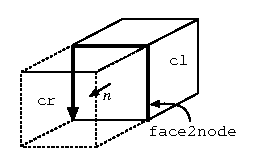
\includegraphics[width=3in]{figures/face.eps}}
%  \epsfxsize=3in
%  \epsfbox{figures/face.eps}}
 \caption{The {\tt face2node} map and its relationship to neighboring cells}
 \label{face2node}
\end{figure}

All boundary faces have a map variable called {\tt ref} that refers to
a common entity that represents the boundary surface.  The name of
each boundary surface is provided in the the {\tt boundary\_name}
fact.  These two variables can be used to assign boundary conditions
as will be described in the following section.  Finally the constraint
{\tt geom\_cells} is a set that contains all geometrically defined
({\it i.e.} physical) cells in the grid, while the constraint {\tt
  cells} contains all cells including non-physical ``ghost'' cells
created at the boundary.

\begin{table}[htbp]
\label{fvmfacts}
\caption{ A Summary of Facts Describing the 3-D finite-volume mesh.}
\begin{center}
  \begin{tabular}{|l|l|l|l|}
    \hline
    Fact  & Type & Location & Description\\
    \hline\hline
    {\tt pos} & {\tt store<vector3d>} & nodes & Node Positions\\
    {\tt face2node} & {\tt multiMap} & faces & Nodes that form a
    face\\
    {\tt cl} & {\tt Map} & faces & cell left of face\\
    {\tt cr} & {\tt Map} & faces & cell right of face\\
    {\tt ref} & {\tt Map} & boundary faces & map to referring category\\
    {\tt boundary\_names} & {\tt store<string>} & boundary categories & boundary category name\\
    {\tt geom\_cells} & {\tt constraint} & physical cells & set of actual cells\\
{\tt cells} & {\tt constraint} & cells & cells including ghost cells\\
    \hline
  \end{tabular}
\end{center}
\end{table}

\subsection{ Setting boundary conditions}

When developing solvers for unstructured grids, it is useful for the
user to specify information that will be associated with various
boundary conditions.  For example, in the heat solver we may wish to
provide an adiabatic and a specified temperature (Dirichlet) boundary
condition.  This can be accomplished by using the {\tt
  boundary\_conditions} variable in the vars file.  This variable will
assign boundary conditions to the various boundary names.  For
example, the {\tt vars} file input
\begin{verbatim}
boundary_conditions: <
 BC_1=adiabatic, BC_2=adiabatic, // opposing slice faces
 BC_3=adiabatic, BC_4=adiabatic, // Two symmetry planes
 BC_5=specified(Twall=300K),     // inner surface
 BC_6=specified(Twall=3000K)     // outer surface
>
\end{verbatim}
would specify that some of the boundary surfaces, namely those
identified as {\tt BC\_1}, {\tt BC\_2}, {\tt BC\_3}, and {\tt BC\_4}
will be have adiabatic boundary conditions, while two boundary
surfaces, {\tt BC\_5} and {\tt BC\_6} will be given specified
temperatures.  Loci provides the {\tt setupBoundaryConditions}
subroutine for parsing this {\tt vars} file input to create
constraints that can be used by Loci rules to apply boundary
conditions.  This is created by calling the subroutine as follows:
\begin{verbatim}
   setupBoundaryConditions(facts) ;
\end{verbatim}
This routine parses the {\tt boundary\_conditions} variable and sets
up constraints with the name of the assigned boundary condition with
an appended ``{\tt \_BC}''.  Thus after this routine is called the
constraints {\tt adiabatic\_BC} is created that contains all of the
faces of {\tt BC\_1} through {\tt BC\_4}, while the constraint {\tt
  specified\_BC} is created to contain all of the faces of {\tt BC\_5}
and {\tt BC\_6}.  In addition, a constraint is created called {\tt
  Twall\_BCoption} that contains the {\bf surface entities} associated with
{\tt BC\_5} and {\tt BC\_6}.  These constraints indicate that it will
be safe to extract these values from the options list that is created
called {\tt BC\_options}.  Thus, we can extract the value of {\tt
  Twall} by using a rule such as the following:
\newpage
\begin{verbatim}
// Extract Twall from boundary condition options
$rule pointwise(Twall<-BC_options),constraint(Twall_BCoption) {
  $BC_options.getOptionUnits("Twall","kelvin",$Twall) ;
}
\end{verbatim}

Once we have extracted the boundary option specified by the user, this
value can then be used to enforce the boundary condition.  For
example, if we wanted to set the face temperature, {\tt
  temperature\_f}, for the specified boundary conditions we would use
the following:
\begin{verbatim}
// Temperature at wall set to specified condition
$rule pointwise(temperature_f<-ref->Twall),constraint(specified_BC) {
  $temperature_f = $ref->$Twall ;
}
\end{verbatim}

\subsection{ Creating matrix data-structures}

Before we begin to make a query, we will need to setup the matrix data-structures that will be used by the linear system solvers.  We do that with the following call:
\begin{verbatim}
   createLowerUpper(facts) ;
\end{verbatim}
This subroutine call will install the multiMaps ``upper'' and
``lower'' into the fact database that are created by transposing the
``cl'' and ``cr'' maps respectively.  These two data-structures
represent the upper and lower triangular portions of the matrix as
will be explained in the matrix assembly section that follows.  We
would also mention that many utilities in the finite-volume module
make use of these maps, so it would be a good idea to make this call
when you plan on using the ``fvm'' module as we are in this example.


\section{Computing the residual function}

The first step in computing the residual function, $R(Q)$ is to
compute the integrated flux through any given face.  This is the term
inside of the summation of equation (\ref{fvmresidual}).  This
equation can easily be evaluated using the rules available through the
``fvm'' module which can provide the areas, normal vectors, and
gradients required.  The variable {\tt area} provides both the normal
vector ({\tt \$area.n}) and the magnitude ({\tt \$area.sada} - sada
stands for square root of area dot area).  The gradient at a face is
provided by the parametric variable ({\tt grads\_f(X)}, thus the heat
flux through a face ({\tt qdot}) is computed using the following Loci rule:
\begin{verbatim}
// Compute the heat flux through faces
$rule pointwise(qdot<-conductivity,grads_f(temperature),area) {
  $qdot = $area.sada*$conductivity*dot($grads_f(temperature),$area.n) ;
}
\end{verbatim}

Note that this will compute fluxes at the face and boundaries.
However, if we know the flux a particular kind of boundary face
(e.g. adiabatic walls) then we need to provide an alternative
computation.  This can present a problem for Loci: if there are two
ways to compute {\tt qdot}, which one is correct?  Loci will generate
an error about conflicting rules when such ties exist.  However, we
can tell Loci how to resolve such a conflict by using a priority
specifier in the signature.  For example, if we use {\tt
  adiabatic::qdot} in the output of the signature, then Loci will know
that this form of qdot is a specialized form that is preferred over the
general {\tt qdot}.  Thus we can override the above rule for adiabatic
boundaries, setting the flux identically to zero here, using the rule:
\begin{verbatim}
// Handle Boundary Conditions
// Adiabatic Wall, qdot = 0, grad(temperature) = 0
$rule pointwise(adiabatic::qdot),constraint(adiabatic_BC) {
  $qdot = 0 ;
}
\end{verbatim}
Another note about priority specification.  Priorities form a
hierarchy so that a priority specification overrides any rule without
priority specification.  And we can then override one priority with
another by adding additional names with ``::'' separators.  For
example, {\tt new::adiabatic::qdot} could be used to override
{\tt adiabatic::qdot}.  However, {\tt specified::qdot} would not override
{\tt adiabatic::qdot} because both have the same priority level.

Note that we have computed the fluxes for each face, however the
computation described in equation (\ref{fvmresidual}) is a sum for
each cell over all the faces of that given cell.  However, we have
computed values located at the faces in the mesh, not the cells.  How
do we perform the cell based sum?  For this operation we use a local
reduction to reduce the face values to sums over cells.  The basic
idea is to visit all faces and sum the fluxes to their corresponding
left and right cells.  As with all reductions in Loci, this operation
starts with a unit rule that assigns the initial value of the residual
to the identity of our reduction operator.  In this case, we will use
the summation operator, and so this identity is zero.  So we begin the
summation with the following unit rule:
\begin{verbatim}
// Add up contributions from all faces, only define qresidual for geom_cells
$rule unit(qresidual),constraint(geom_cells) {
  $qresidual = 0 ;
}
\end{verbatim}

To complete the summation, we must now visit each cell and add its
contribution to the left and right sides.  For each face we use the
{\tt join} method to add {\tt qdot} to the left cell residual.  Then
we do the same for the right side of faces.  However, we note that
since the face is oriented such that the normal points into the right
side, we must change the sign of qdot before adding into the residual
on this side.  Also note that we could have used the {\tt +=} operator
instead of using {\tt join}, however using join is preferred as it
guarantees that we are using the selected operator (in this case {\tt
  Loci::Summation}).  If you aren't consistent in the use of operators
with apply rules, you may get inconsistent results, particularly when
running in parallel.
\begin{verbatim}
// Add to left cell
$rule apply(cl->qresidual<-qdot)[Loci::Summation],
  constraint(cl->geom_cells) {
  join($cl->$qresidual,$qdot) ;
}

// Add to right cell, note sign change due to normal pointing into cell
$rule apply(cr->qresidual<-qdot)[Loci::Summation],
  constraint(cr->geom_cells) {
  join($cr->$qresidual,-$qdot) ;
}
\end{verbatim}

Note that in order to compute the gradient of temperatures as is
required in the first rule that computes {\tt qdot}, that we need to
also provide values for temperatures at the boundary faces.  This is
provided through the variable {\tt temperature\_f}.  Note, that in
general if we want to find the gradient of variable {\tt X}, then the
variable {\tt X\_f} needs to also be defined at the boundary faces.  We
derive the boundary temperature based on the boundary condition.  For
an adiabatic wall we just use the cell temperature inside as the wall
temperature.  Since the temperature of the cell next to the boundary
is on the left side of the boundary face (all boundary faces have
normals pointing out of the domain), then we simply set the wall
temperature to {\tt cl->temperature}, as we do in the following rule:

\begin{verbatim}
// Compute boundary temperatures
// adiabatic,  dT/dx = 0, so copy temperature from cell to face
$rule pointwise(temperature_f<-cl->temperature),constraint(adiabatic_BC) {
  $temperature_f = $cl->$temperature ;
}
\end{verbatim}

For a temperature specified wall, we simply set the boundary face
temperature to the user specified value.  We can get this value using
the {\tt ref} map, provided that a rule to extract this from
{\tt BC\_options} has already been provided (see previous section on boundary
conditions).  Thus for the specified temperature boundary condition,
we compute the temperature with the following rule:

\begin{verbatim}
// Temperature Specified Wall
$rule pointwise(temperature_f<-ref->Twall),constraint(specified_BC) {
  $temperature_f = $ref->$Twall ;
}
\end{verbatim}

We have now described how to compute the residual.  Now we need to
assemble the matrix on the left-hand-side of equation
(\ref{fvmscheme}) to complete the solver.  This is described in the
next section.

\section{Assembling the matrix}

Before describing the assembly of the matrix, lets first begin with
the computation of derivatives of the face fluxes with respect to the
variables at each side.  However, to properly describe the matrix, we
will need to have some idea of how the gradient function is
implemented.  For the purpose of assembling the Jacobian, we will use
the following approximation of the flux function, which will be a
reasonable approximation for most grids of reasonable quality.  Note
the flux function is expressed as
\begin{equation}
\dot{q} = \mathcal{A}_f k \left( \nabla T_f \cdot \vec{n}_f\right) \approx \mathcal{A}_f k \left(\frac{T_l-T_r}{(\vec{x}_l-\vec{x}_r)\cdot \vec{n}_f}\right),
\end{equation}
where $T_l$, $x_l$, $T_r$, and $x_r$ are the temperatures and cell
centroids of the left and right side of the face respectively.  Given
this, we can then determine the derivatives of this flux with respect
to the left and right conservative variable values.  Thus we arrive at
the following derivatives:
\begin{equation}
\frac{\partial \dot{q}}{\partial Q_l} = \frac{\partial \dot{q}}{\partial T_l} \frac{\partial T_l}{\partial Q_l} = \frac{\mathcal{A}_f k }{(\vec{x}_l-\vec{x}_r)\cdot \vec{n}_f}\frac{\partial T_l}{\partial Q_l},
\end{equation}
and
\begin{equation}
\frac{\partial \dot{q}}{\partial Q_r} = \frac{\partial \dot{q}}{\partial T_r} \frac{\partial T_r}{\partial Q_r} = -\frac{\mathcal{A}_f k }{(\vec{x}_l-\vec{x}_r)\cdot \vec{n}_f}\frac{\partial T_r}{\partial Q_r}.
\end{equation}

These derivatives are easily implemented as Loci rules such as the following:
\begin{verbatim}
// Derivative of flux from left side
$rule pointwise(dqdotdQl<-conductivity,(cl,cr)->cellcenter,area,cl->dTdQ) {
  real distance = dot($cl->$cellcenter-$cr->$cellcenter,$area.n) ;
  $dqdotdQl = $area.sada*$conductivity*$cl->$dTdQ/distance ;
}

// Derivative of flux from right side
$rule pointwise(dqdotdQr<-conductivity,(cl,cr)->cellcenter,area,cr->dTdQ) {
  real distance = dot($cl->$cellcenter-$cr->$cellcenter,$area.n) ;
  $dqdotdQr = -$area.sada*$conductivity*$cr->$dTdQ/distance ;
}
\end{verbatim}

Note, however, that these derivatives only apply at the interior faces
where {\tt cellcenter} exists on both sides of the face.  We need
separate derivations for the derivatives of the flux at the boundary
faces.  here we implement two obvious boundary conditions flux
derivatives that follow easily from the above formulations:

\begin{verbatim}
// derivatives of boundary flux for specified temperature wall
$rule pointwise(dqdotdQl<-conductivity,facecenter,cl->(cellcenter,dTdQ),area),
  constraint(specified_BC) {
  real distance = dot($cl->$cellcenter-$facecenter,$area.n) ;
  $dqdotdQl = $area.sada*$conductivity*$cl->$dTdQ/distance ;
}

// derivative of boundary flux for adiabatic wall (zero)
$rule pointwise(dqdotdQl),constraint(adiabatic_BC) {
  $dqdotdQl = 0 ;
}
\end{verbatim}

Before describing how to assemble these derivatives into a system
matrix, we should spend a little more time describing data-structures
that were created by the call to {\tt setupFVMGrid} and to {\tt
  createLowerUpper}.  While the topology of the face2node map has
already been discussed, it should be noted that the selection of the
local face coordinates could be considered arbitrarily.  However, in
the Loci finite-volume tools, we have a specific method of choosing
this ordering: specifically the faces are oriented so that the normals
point from a lower equation number to a higher equation number.  This
allows us to associate the matrix non-zero structure directly with the
mesh data-structure.  Thus, when we invert the {\tt cr} map we get a
map that corresponds to the lower triangular part of the system
matrix, where the off-diagonal components are stored at the faces.
Similarly, the inverse of the {\tt cl} map provides us with the upper
triangular part of the system matrix.  We can now describe the system
matrix using the left and right flux derivatives located at the faces
that form the L and U components of the system matrix, supplementing
this with a diagonal element, D, stored at the cells.  This is
illustrated in figure \ref{cellperspective} which shows the flux
Jacobians from the left and right sides (denoted as fjp and fjm
respectively) located at the cells, and the D entries associated with
the cell.  Alternatively, one can look at figure
\ref{matrixperspective} to get the matrix assembly view.  Here we see
that along a row the {\tt lower} map can be used to access the lower
non-zero elements, while the corresponding {\tt cl} map can be used to
find the corresponding equation with that non-zero entry.  A similar
procedure is used to describe the upper matrix, only using the {\tt
  upper} map and {\t cr} to accomplish the same goal. This provides us
with a convenient representation of the assembled matrix.


\begin{figure}[htbp]
 \centerline{
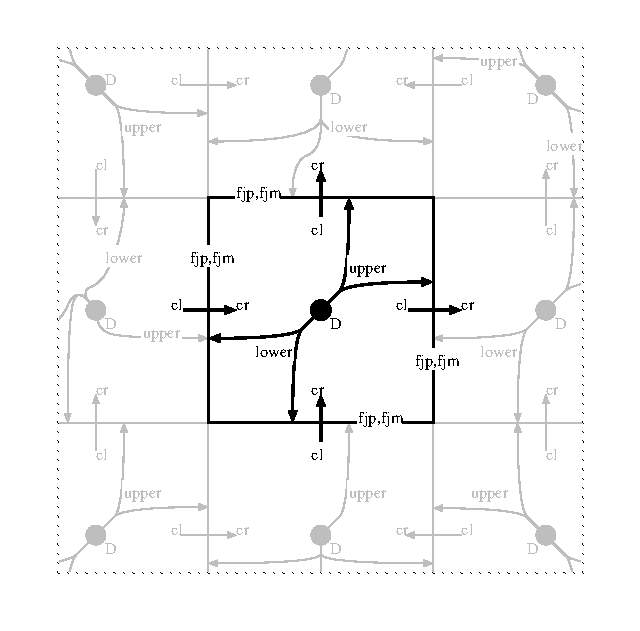
\includegraphics[width=2.4in]{figures/cell.eps}}
%  \epsfxsize=2.4in
%  \epsfbox{figures/cell.eps}}
 \caption{Upper and lower maps viewed from the cell}
\label{cellperspective}
\end{figure}

\begin{figure}[htbp]
 \centerline{
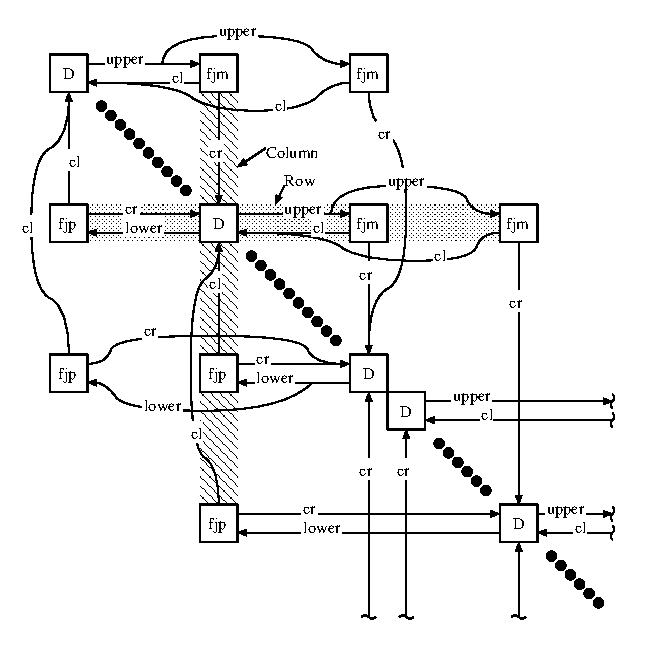
\includegraphics[width=4.5in]{figures/mat.eps}}
%  \epsfxsize=4.5in
%  \epsfbox{figures/mat.eps}}
 \caption{Matrix Data-Structure as used by the finite-volume module}
\label{matrixperspective}
\end{figure}
%\clearpage
\subsection{And now the assembly}

Now we can describe the procedure for assembling the linear system.
First we provide the overall linear system with a name that will be
used to collect the different parts of the system.  For example, lets
call this system the {\tt heat} system of equations.  Then we form the
linear system by creating the variables {\tt heat\_B} for the
right-hand-side, and {\tt heat\_L}, {\tt heat\_U}, and {\tt heat\_D}
for the system matrix, $A=L+D+U$.  First the creation of heat\_B is
straightforward as it is just the residual function.  This is easily
implemented as:
\begin{verbatim}
$rule pointwise(heat_B<-qresidual) {
  $heat_B = $qresidual ;
}
\end{verbatim}

The computation of the diagonal term is somewhat more complex.  The
diagonal term will involve the derivatives of the fluxes (with
appropriate sign changes to account for normal vector orientation),
plus the term that appears due to the time derivative.  We perform
this operation with two steps.  First we compute the sum of all
diagonal contributions from the flux derivatives using a local
reduction similar to what was done for the residual evaluation.
However, in this case we have to select the derivative side so that
it results in a diagonal contribution.  This is accomplished with the
following code:

\begin{verbatim}
// To compute the diagonal term, we first must sum the diagonal
// contributions from the flux derivatives.
$type sumDiagonal store<real> ;

// Add up diagonal contributions from flux derivatives
$rule unit(sumDiagonal), constraint(geom_cells) {
  $sumDiagonal = 0 ;
}

// Add contribution from face to left cells
// (e.g. d R(Ql,Qr)/d Ql goes to diagonal of the left cell)
$rule apply(cl->sumDiagonal<-dqdotdQl)[Loci::Summation],
  constraint(cl->geom_cells) {
  join($cl->$sumDiagonal,$dqdotdQl) ;
}

// Add contribution from face to right cells 
// (e.g. d R(Ql,Qr)/d Qr goes to diagonal of the right cell)
// Note sign change due to normal pointing into the cell
$rule apply(cr->sumDiagonal<-dqdotdQr)[Loci::Summation],
  constraint(cr->geom_cells) {
  join($cr->$sumDiagonal,-$dqdotdQr) ;
}
\end{verbatim}

We can now form the diagonal term of the matrix with the
straightforward Loci pointwise rule:
\begin{verbatim}
$rule pointwise(heat_D<-sumDiagonal,deltaT,vol) {
  $heat_D = $vol/$deltaT - $sumDiagonal ; 
}
\end{verbatim}
Note, that it would be tempting to put the term {\tt \$vol/\$deltaT}
into the unit rule of $sumDiagonal$ to save a rule implementation.
However such an approach would be incorrect as Loci expects the unit
rule to initialize the variable to the identity of the reduction
operator.  Since this value would not be the identity, some of the
reasoning that Loci uses to prove programs, in particular parallel
programs, would be incorrect.  Note, that it would be possible to
combine this with the reduction by having another apply rule add in
the {\tt vol/deltaT} term. However, this would be provided by an
additional apply rule, not the unit rule.


To finish the assembly of the linear system we need to describe the
upper and lower triangular portions of the matrix.  Note that for the
description of these terms we need to carefully consider the signs of
the resulting system.  Recall that the system matrix subtracts the
flux derivatives, and we also need to take into consideration the sign
changes due to normal vector compatibility with the divergence
theorem.  Here is the logic:  The lower portion of the matrix consists
of derivatives of fluxes that were summed into the current cell
through it's {\tt cr} map with respect to the cell $Q$ on the left
side of this face.  Because this was summed with a change of sign due
to the normal pointing into the cell, and the subtraction in the system
matrix, this term is $- (- (\frac{\partial \dot{q}}{\partial Q_l}))$.
The upper off-diagonal terms, by similar argument, will be $-
(\frac{\partial \dot{q}}{\partial Q_r})$.  The following rules define
the off-diagonal parts of the matrix and complete the assembly of the
linear system.
\begin{verbatim}
// Compute matrix lower term from flux derivatives
// Note, we are subtracting del R/del Q in the matrix so there is an extra
// sign change here
$rule pointwise(heat_L<-dqdotdQl) {
  $heat_L = $dqdotdQl; 
}

// Compute matrix upper term from flux derivatives
$rule pointwise(heat_U<-dqdotdQr) {
  $heat_U = -$dqdotdQr;
}
\end{verbatim}

Now that we have formed the linear system, we can use a parametric
rule from the ``fvm'' module to use the PETSc toolkit to solve the
linear system by using the following rule:
\begin{verbatim}
// Solve linear system described by heat_B, heat_D, heat_L, heat_U
$rule pointwise(deltaQ<-petscScalarSolve(heat)) {
  $deltaQ = $petscScalarSolve(heat) ;
}
\end{verbatim}

\section{Performing the time integration}

Now we have nearly all of the components in place to build the
implicit time integration method.  The completion of this process
follows the same lines as the explicit Euler integration provided in
the one-dimensional example.  We begin this time-stepping method by
building the first iteration value for the conservative variable.
This is accomplished using the following ``build'' rule:
\begin{verbatim}
// Initial Conditions
$rule pointwise(Q{n=0}<-Density,Cp,T_initial) {
  $Q{n=0} = $Density*$Cp*$T_initial ;
}
\end{verbatim}
Now that we have $Q^{n=0}$ defined, we can iterate by simply defining
how to get from $Q^n$ to $Q^{n+1}$.  This step is trivial using the
{\tt deltaQ} computed in the previous section.  The ``advance'' rule
that does this is specified as:
\begin{verbatim}

// Advance the timestep using linear system solution
$rule pointwise(Q{n+1}<-Q{n},deltaQ{n}), constraint(geom_cells) {
  $Q{n+1} = $Q{n}+ $deltaQ{n} ;
}
\end{verbatim}

The specification so far gives us the ability to iterate forward in
time, but provides no provisions for terminating the iteration.  We
must provide the conditions of termination and a ``collapse'' rule
that tells Loci what to do in the event of termination.  We compute
the condition for termination by detecting when a user provided stop
iteration has been reached with the following rule:
\begin{verbatim}
// Determine when we will finish timestepping
$rule singleton(finishTimestep<-$n,stop_iter) {
  $finishTimestep = ($$n > $stop_iter) ;
}
\end{verbatim}

We can now specify how to collapse the iteration.  In this case, we
collapse to the variable {\tt solution} which is the generic query
that we usually make for Loci applications.  This query plays the same
sort of role as {\tt main} in a C program in that it provides us a
standard place to start a Loci program.  The collapse rule is simply
implemented as described below:
\begin{verbatim}
// Collapse to solution when we are finished iterating
$rule pointwise(solution<-Q{n}),conditional(finishTimestep{n}),
  constraint(geom_cells) {
  $solution = $Q{n} ;
}
\end{verbatim}

\section{Closing the equations}

At this stage, the solution to the time dependent heat equation is not
quite in place.  While we have described how to compute {\tt deltaQ},
the computation of this variable requires the computation of {\tt
  qdot}, which in turn requires a definition for {temperature}.  So far
we have described how the conservative variable $Q=\rho e$ evolves in
time, but we have not related this to temperature.  We can do this by
using the relationship that $e = C_p T$, thus $T = Q/(\rho C_p)$.  We
can use this relationship to establish the temperature as a function
of {\tt Q} with the rule:
\begin{verbatim}
// Compute temperature from energy
$rule pointwise(temperature<-Q,Density,Cp), constraint(geom_cells) {
  $temperature = $Q/($Density*$Cp) ;
}
\end{verbatim}
In addition to the temperature, we also needed the transformational
derivative $\frac{\partial T}{\partial Q}$ in order to compute the
system matrix.  This is provided by the following rule:
\newpage
\begin{verbatim}
// Compute transformation derivative from temperature to Q
$rule singleton(dTdQ<-Density,Cp) {
  $dTdQ = 1./($Cp*$Density) ;
}
\end{verbatim}
At this point, we will be able to solve the three-dimensional heat
equation in a form that is automatically parallelizable.

\section{Creating plot files}

So far we have developed a solver, but even though the solution is
time-dependent, we only get to see the final ``solution'' that is
placed in the fact database, when we would like to view the time
evolution of the solution.  Loci provides a facility whereby rules can
be executed as the time-stepping algorithm proceeds.  We can do this
by creating a variable that computes a special variable called {\tt
  OUTPUT}.  The variable {\tt OUTPUT} is a special variable that is
automatically requested in all iteration loops.  If the variables that
are input to the rule are being evaluated in the iteration, then this
rule will be executed.  For example, suppose that we wish to display
the steady residual each time-step, then we could implement a rule such
as:
\begin{verbatim}
$rule singleton(OUTPUT<-L2Norm(qresidual),$n),
  option(disable_threading) {
  if(Loci::MPI_rank==0) {
    cout << "R" << $$n << ": " << $L2Norm(qresidual) << endl ;
  }
}
\end{verbatim}
Lets note several important artifacts about this rule.  First note
that the signature indicates that the result of the computation is a
variable called {\tt OUTPUT} which indicates that the main purpose of
this rule will be to have some effect on the outside world. The rule
is inputing the variable {\tt L2Norm(qresidual)} which results in the
computation of the volume integrated L2-norm of the steady state
residual, {\tt qresidual}.  The rule also inputs the current time-step
{\tt \$n} so that it can report it along with the residual output.
Also note the conditional on {\tt Loci::MPI\_rank} equal to zero.
This conditional statement is there to prevent multiple outputs from
each processor when running in parallel.  Also note the use of the
option {\tt disable\_threading}.  This option tells Loci that this
rule is sensitive to the order that computations occur, and to make
sure not to do any optimizations that would cause the computation to
be called multiple times.

Now we can see how to print simple output to the screen, but how do we
get a chance to make a plot of the simulated temperature field?  We
can perform a similar operation by using Loci's built in facility to
read/write containers (in parallel or serial) to a portable HDF5 file.
An example of such a rule follows:

\newpage
\begin{verbatim}
$rule pointwise(OUTPUT<-cell2node(temperature),$n,plot_modulo),
  constraint(pos),conditional(doPlot), option(disable_threading),
  prelude {
  int iter = *$$n % *$plot_modulo ;
  ostringstream oss ;
  string varname = "temperature" ;
  oss << "output/" << varname << "_hdf5." << iter ;
  string filename = oss.str() ;

  if(Loci::MPI_rank == 0)
    cout << "writing file " << filename << endl ;

  // Create an hdf5 file
  hid_t file_id = Loci::hdf5CreateFile(filename.c_str(),H5F_ACC_TRUNC,
                                       H5P_DEFAULT,H5P_DEFAULT) ;

  // Write the values of the nodal temperatures into the file
  Loci::writeContainer(file_id,varname,$cell2node(temperature).Rep()) ;

  // Close the hdf5 file
  Loci::hdf5CloseFile(file_id) ;
} ;
\end{verbatim}
In this rule we output the special variable {\tt OUTPUT} which
indicates that this rule will be executed if the inputs are being
computed in the given iteration.  The rule inputs the parametric
variable {\tt cell2node(temperature)} which will interpolate from the
cell values of {\tt temperature} and the boundary face values {\tt
  temperature\_f}.  We constrain the rule to apply to all entities that
have a value for {\tt pos} (which are the nodes in the mesh), and we
add the option {\tt disable\_threading} which makes sure that all
processors will act on this rule in a synchronized and indivisible
manner.  An important thing to note is the existence of the {\tt
  prelude} keyword is indicating that we are describing activities
that operate on the containers (usually as a prelude to computations),
rather than the values contained within the containers.  We need this
keyword because we are about to write the {\it containers} to a file.
In the prelude, when we access a particular variable, we are not
accessing the contents, but rather the container itself.  Thus, to
access the value of the parameter {\tt plot\_modulo} we use the {\tt
  *} operator ({\it e.g.} {\tt *\$plot\_modulo}.  In this particular
case, we write the file out into the ``output'' directory with a name
that is compatible with using the ``extract'' post processing
utility.  We write the container out using the {\tt writeContainer}
function, and note that we use the {\tt .Rep()} method to get the
abstract representation of the container to pass to this routine.
Finally, note that we have placed a conditional execution argument on
this rule (conditional execution statements can be placed on collapse
rules that end iterations or rules that output the variable {\tt
  OUTPUT}).  This conditional statement is to allow us to only
occasionally write out this file.  We provide a separate rule to
compute the conditional variable ({\tt doPlot}) as implemented below:
\newpage
\begin{verbatim}
// Compute when we want to make plot files
$type doPlot param<bool> ;

$rule singleton(doPlot<-$n,plot_freq) {
  $doPlot = (($$n % $plot_freq) == 0) ;
}
\end{verbatim}

\section{Running the solver}

The heat solver described can be used to solve the heat equation on
general unstructured grids, and can exploit massively parallel
distributed memory clusters.  The source code to a complete heat
solver is provided in the {\tt heat} directory of the tutorial.  A
test grid and vars file has been included in the directory for your
experimentation.  To run the example case use the command
\begin{verbatim}
mpirun -np 1 ./heat test
\end{verbatim}

Note you can also look at the schedule that is generated by Loci using
the {\tt --scheduleoutput} option.  The {--nochomp} option disables
the chomping optimization which may make the schedule easier to
understand.  For example to see the schedule generated by Loci run
\begin{verbatim}
mpirun -np 1 ./heat --scheduleoutput --nochomp test
\end{verbatim}

The heat solver will dump plot files into the {\tt output}
subdirectory. A post-processing tool called {\tt extract} can be used
to convert these files into a format that can be visualized by various
visualization packages including {\it ensight}, {\it fieldview}, and
{\it tecplot}.  For example to see the results of the simulation after
10 iterations using ensight, one enters the command:
\begin{verbatim}
extract -en test 10 ntemperature
\end{verbatim}
This creates a directory {\tt ensight\_test} that contains an ensight case
file for visualization of the solution results.  The argument
ntemperature tells extract that you want to extract the nodal plot
variable {\tt temperature} that is stored in the {\tt output
  directory}.  Use {\tt extract -help} for more information.

\chapter{Using storeVec and storeMat}

Loci provides facilities for having vectors and matricies that have a
size that is not known until the program executes.  This facility
would be used, for example, when the number of chemical species is not
known until specified by the user, or other applications where the
size of inforation stored at each entity could be specified by user
input.  For these applications we have the containers {\tt storeVec}
and {\tt storeMat}.  These containers have a method {\tt setVecSize()}
that must be called before values are written to the container.
Generally this method will be required for pointwise and unit rules
that are responsible for creating {\tt storeVec} or {\tt storeMat}
containers.  Below is an example of a rule that computes a {\tt storeVec}:
\begin{verbatim}
  $type Ivec storeVec<double> ;
  $type numBands param<int> ;
  $type Omegas param<vector<double> > ;

  $rule pointwise(Ivec{n=0}<-numBands,Omegas),constraint(geom_cells),
    prelude {
    $Ivec{n=0}.setVecSize(*$numBands*(*$Omegas).size()) ;
  } compute {
    $Ivec{n=0} = mk_Scalar(0) ;
  }
\end{verbatim}
Note that this code includes a {\tt prelude} block and a {\tt compute}
block.  The prelude block operates on the containers and is executed
before the compute block.  The compute block describes, like most Loci
rules, what to do for each entity that satisfies the rule signature.
In other words, the {\tt compute} block operates on values, while the
{\tt prelude} block operates on the containers.

The {\tt storeVec} container creates array of values for each entity.
In general you can assign or ues the {\tt +=}, {\tt-=}, {\tt \*=}, or
{\tt /=} operators with these arrays.  The {\tt mk\_Scalar()} function in
the above code converts a scalar value to a vector with the same
scalar value repeated for each entity.  These operators facilitate a
straightforward approach to operating on arrays and matricies.
However, it is also perfectly acceptable to operate on the individual
vector entries using the array operator, ({\tt []}), such as
demonstrated with a rewrite of the above rule shown below:
\begin{verbatim}

  // An equivalent variation of the above code
  $rule pointwise(Ivec{n=0}<-numBands,Omegas),constraint(geom_cells),
    prelude {
    $Ivec{n=0}.setVecSize(*$numBands*(*$Omegas).size()) ;
  } compute {
    const int vs = $numBands*$Omegas.size() ;
    for(int i=0;i<vs;++i) // Loop over vector and set each entry to zero
      $Ivec{n=0}[i] = 0 ;
  }
\end{verbatim}


\chapter{Debugging Hints}

Debugging techniques for Loci programming is both similar to and
different from standard programming methods.  First you can use
debuggers such as {\tt gdb} on Loci programs, although you may want to
edit the Makefile to include a line to enable the debugging option and
recompile.  The line you will add is given as:
\begin{verbatim}
COPT = -g
\end{verbatim}
In addition, after {\tt Loci::Initialize()} you can call the function
{\tt set\_fpe\_abort()} which will cause floating point exceptions to
abort the program.  In addition, for parallel programs, you can get
Loci to automatically create terminal windows with debuggers running
on any processes that aborted if you call the program with the
following options:
\begin{verbatim}
heat --display $DISPLAY --debug gdb test
\end{verbatim}

In Loci programs, you frequently need to understand why a rule isn't
being included in a schedule, or why a schedule is not being formed.
There are several techniques that are useful for figuring out what is
going on in the Loci schedule.  Probably the most useful file in this
regard is the files dumped into the {\tt debug/} directory.  These
files contain descriptions of rules that were removed from the
schedule with an explanation of why ({e.g.} what information was
missing that made it impossible to execute that rule).  This is often
very useful in determining what is going on.  In addition, it is
usually helpful to examine the schedule files created when using the
option {\tt --scheduleoutput}.  Usually this is more useful when
combined with the {\tt --nochomp} option that disables some
optimizations that may make the schedule hard to read.  Usually
inspections of the schedule are targeted in that we are looking for a
particular rule, when it is executed and over what entities.

In addition to the above techniques, there are several ways that we
can use the Loci scheduler to help identify problems.  The first is to
use constraints.  If a rule is being used in a schedule, but not over
the entities expected, it can be useful to temporarily add a
constraint to force the rule to be executed over a particular set of
entitites.  For example, if a value should be available for all faces,
adding {\tt constraint(area)} will force Loci to tell you what
variables kept the rule from satisfying the constraint.  However, in
general it is a good idea to use constraints in a limited fashion, as
in the end a constraint limits the way in which a rule might be used.
So, once the debugging is finished it is a good idea to remove any
unnecessary constraints. 

Another approach is to add dummy rules to shortcut part of the
computations.  For example, in the heat solver if we are wondering why
the advance rule isn't being called, we could add rules that we know
can be scheduled to fill in part of the code.  For example, we could
shortcircuit the {\tt deltaQ} computation with the rule:
\begin{verbatim}
$rule pointwise(deltaQ<-Q) {
// Dummy rule to check for schedule consistency
} 
\end{verbatim}
If Loci is able to generate a reasonable schedule, you can then change
the inputs to the rule to discover where the computations were having
trouble.  For example changing the rule to the following would check
to see that we were able to derive the variable {\tt heat\_B}:
\begin{verbatim}
$rule pointwise(deltaQ<-heat_B) {
// Dummy rule to check for schedule consistency
} 
\end{verbatim}


%% Appendicies
\appendix

\chapter { Makefile Example}
\label{chap:makefile}
Compiling Loci programs is easy if you copy the make file from the
heat example directory in the tutorial and adapt it to your
application.  All that is needed is to edit {\tt LOCI\_BASE} to point
to the directory where Loci is installed, let {\tt OBJS} point to a
list of the object files that will be compiled into your final
executable.  Finally, use the {\tt TARGET} variable to set the
executable name.  The makefile is given as a reference on the
following page.

\include{Makefile_ex}

\chapter{The {\tt fvm} Module Services}

\section{Grid Metrics}

\begin{center}
\begin{tabular}[h]{|l|l|}
\hline
{\tt cellcenter} & Cell Centroid\\
{\tt vol} & Cell Volume\\
{\tt facecenter} & Face Centroid\\
{\tt area} & Face Area and Normal\\
{\tt grid\_vol} & Total Grid Volume\\
\hline
\end{tabular}
\end{center}

\section{Spatial Gradients}

\begin{center}
\begin{tabular}[h]{|l|l|}
\hline
{\tt grads(X)} & Scalar Gradient at Cell \\
{\tt gradv(X)} & Vector (array) Gradient at Cell\\
{\tt gradv3d(X)} & 3-D Vector Gradient at Cell\\
{\tt grads\_f(X)} & Scalar Gradient at Face\\
{\tt gradv\_f(X)} & Vector (array) Gradient at Face\\
{\tt gradv3d\_f(X)} & 3-D Vector Gradient at Face\\
\hline
\end{tabular}
\end{center}

\section{Face Extrapolations}

\begin{center}
\begin{tabular}[h]{|l|l|}
\hline
{\tt lefts(X)} & Scalar Extrapolation to Face Left Side \\
{\tt rights(X)} & Scalar Extrapolation to Face Right Side \\
{\tt leftsP(X,M)} & Bounded Scalar Extrapolation to Face Left Side \\
{\tt rightsP(X,M)} & Bounded Scalar Extrapolation to Face Right Side \\
{\tt leftvM(X)} & Mixture Extrapolation to Face Left Side \\
{\tt rightvM(X)} & Mixture Extrapolation to Face Right Side \\
{\tt leftv3d(X)} & 3-D vector Extrapolation to Face Left Side \\
{\tt rightv3d(X)} & 3-D vector Extrapolation to Face Right Side \\
\hline
\end{tabular}
\end{center}

\section{Nodal Interpolations}

\begin{center}
\begin{tabular}[h]{|l|l|}
\hline
{\tt cell2node(X)} & interpolate scalar to mesh nodes \\
{\tt cell2node\_v(X)} & interpolate vector to mesh nodes \\
{\tt cell2node\_v3d(X)} & interpolate 3-D vector to mesh nodes \\
{\tt cell2nodeMax(X)} & mesh nodes get maximum neighbor value \\
{\tt cell2nodeMin(X)} & mesh nodes get minimum neighbor value \\
{\tt cell2nodeMaxMag(X)} & mesh nodes get maximum magnitude neighbor value \\
{\tt cell2nodeMaxv3d(X)} & Maximum neighboring 3d value \\
\hline
\end{tabular}
\end{center}


%\section{Surface Integrations}


\section{Linear System Solvers}

\begin{center}
\begin{tabular}[h]{|l|l|}
\hline
{\tt petscScalarSolve(X) } & solve linear system one dof per cell \\
{\tt petscBlockedSolve(X) } & solve linear system with many dof per cell (double input)\\
{\tt petscBlockedSSolve(X) } & solve linear system with many dof per cell (float input)\\
\hline
\end{tabular}
\end{center}

\section{Basic Norms}

\begin{center}
\begin{tabular}[h]{|l|l|}
\hline
{\tt L1Norm(X)} & Volume Integrated L1-norm \\
{\tt L2Norm(X)} & Volume Integrated L2-norm \\
{\tt LinfNorm(X)} & Infinity Norm \\
\hline
\end{tabular}
\end{center}



\chapter{Datatypes }
%
\section {Introduction}
For the purpose of I/O and communication, datatypes can be considered
as abstract representations of the state of an object.  Usually this
is represented by the memory locations where data is stored.  In the
Loci framework, we gave to specify how to save and restore the state
of new object types explicitly to facilitate interprocessor
communication in heterogeneous environments or portable file I/O.
This information is provided to Loci using the traits mechanism.

In Loci, the datatype information is encapsulated in {\tt
  data\_schema\_traits} template class.  A user will need to provide a
specialized template for his/her own datatypes before they can be
used with Loci containers such as {\tt store}.
%
\section {Classification of Datatypes} 

Datatypes could be classified according to the their relationship
between computer memory representation and data which they hold.  The
basic distinction depends on the way C++ stores the object in memory.
If the object is represented in a continuous segment of memory with a
fixed layout, then then the memory layout is consistent with the
schemas used to send messages or write data to files.  If, instead the
objects data is scattered through memory or has a size that is
determined at run time, then the object must be serialized before it
can be sent as a message or placed in file storage.  An object whose
memory layout is compatible with the contiguous memory schema uses an
{\tt IDENTITY\_SCHEMA\_CONVERTER} for serialization.  Other objects
must also specify a schema converter.  The specifics of this will be
specified in the below examples:
%
\begin {verbatim}
typedef struct My_Type_t {
    int       iScalar;
    float     fScalar;
    char      cScalar;
    double    dScalar;
} My_Type1;

typedef struct My_Type_t {
    int        iScalar;
    float      fScalar;:
    char       cScalar;
    double    *dScalar;
} My_Type2;
\end{verbatim}
%
For {\em My\_Type1} C/C++ guarantees that the members of a structure
are stored in contiguous memory locations with some padding, so the
bitwise copy of {\em My\_Type1} will pack the data correctly, whereas
for {\em My\_Type2} the address of {\em dScalar} and not the data will
be copied. In the first case, the memory schema and the file schema is
handled by an {\bf Identity Function} called the {\tt
  IDENTITY\_SCHEMA\_CONVERTER }

In the second case, we need to explicitly convert between memory
schema and the file schema by specifying {\tt USER\_DEFINED\_CONVERTER}.

It should be mentioned here, that pointers are not the only source of
difference between these two datatype. STL container like vector,
list, queues, maps and virtual classes, all would need user to
serialize the state they contains, therefore, they also fall under the
category of user defined converter type.


\section {Predefined Datatypes in Loci}
Loci provides some of the frequently used datatypes so that user need
not write for themselves.These are
%
%
\begin{enumerate}
\item {\bf Atomic Datatype}
As the name implies, these datatypes are indivisible types. These type
are supported by all machines. These are building blocks for all other
datatypes. All native C/C++ datatypes are atomic datatypes
in Loci. The following table provides all the atomic datatypes support
by the Loci.
%
\begin{center}
\begin{tabular} [h] {|l|l|} \hline
Loci Datatype & Native C++ Datatype \\ \hline \hline
BOOL & bool \\ \hline
CHAR & signed char \\\hline
UNSIGNED\_CHAR & unsigned char \\\hline
SHORT & short \\\hline
UNSIGNED\_SHORT & unsigned short \\\hline
INT & int \\\hline
UNSIGNED & unsigned \\\hline
LONG & long \\\hline
UNSIGNED\_LONG & unsigned long \\\hline
FLOAT & float \\\hline
DOUBLE & double \\\hline
\end{tabular}
\end{center}
\item {\bf Array class}
Loci, provides template version of constant size array
\begin{verbatim}
template <class T, unsigned int n>
class Array {
   public:
   .
   .
   private:
      T  x[n];
};
\end{verbatim}
\item {\bf Vector class}
Loci, has 2D/3D vesions of vector class(mathematical vectors)
\begin{verbatim}
 template<T>
 struct vector3d {
      T x,y,z ;
 }

 template<T>
 struct vector2d {
      T x,y ;
 }
\end{verbatim}
\item {\bf STL containers parameterized by types using the {\tt
      IDENTITY\_SCHEMA\_CONVERTER}} 

All standard STL containers with predefined identity schema types are supported.
\begin{enumerate}
\item vector
\item list
\item queue
\item set
\item map
\end{enumerate}
\end{enumerate}
\section {Creating your own compound datatypes}
%
Loci, uses {\tt data\_schema\_traits} template class to determine
the datatype of an object. The generic behavior of template class is
not suitable for identifying or creating new datatype, so we use {\bf
  template Specialization } technique to customize or create new
datatypes . This {\tt data\_schema\_traits} class has one static
member function {\tt get\_type()} in which user specifies the
information about new datatype. A general skeleton for creating new
datatype look as follows
\begin{verbatim}
namespace Loci {
   // Skelton for datatype having identity schema
   template <>
   struct data_schema_traits <My_New_Type1 > {
         typedef IDENTITY_CONVERTER Schema_Converter;
         static DatatypeP get_type() {
                CompoundDatatypeP cmpd = CompoundFactory(My_New_Type1());
                LOCI_INSERT_TYPE(cmpd, My_New_Type1, member);
                   .
                   .
                return DatatypeP(cmpd);
         }
   };
}
\end{verbatim}
%
Where {\bf CompoundFactory} is one of the software design pattern for creating a 
new compound datatype object. Since the allocation of this object is done inside
the functions, the question will always arise, who is responsible for deleting
the object ? To destroy the objects when they are not needed, we use reference counting and the 
{\tt CompoundDatatypeP} class stands for {\em Reference Counting} version of
{\tt CompoundDatatype} class.
%
\par If your C/C++ structures contains members of predefined Loci datatypes, then it
is fairly easy to create corresponding Loci datatype. For example
\begin{verbatim}
 typedef struct My_Compound_Type_t {
        float                       fScalar;      
        vector3d<double>            vect3d;
        Array<double,2>             array1d;
        Array<Array<double,2>,4>    array2d;
 } My_Compound_Type;

 namespace Loci {
  template <> struct data_schema_traits <My_Compound_Type > {
     typedef IDENTITY_CONVERTER Schema_Converter;
     static DatatypeP get_type() {
         CompoundDatatypeP cmpd = CompoundFactory(My_Compound_Type());
         LOCI_INSERT_TYPE(cmpd, My_Compound_Type, fScalar);
         LOCI_INSERT_TYPE(cmpd, My_Compound_Type, vect3d);
         LOCI_INSERT_TYPE(cmpd, My_Compound_Type, array1d);
         LOCI_INSERT_TYPE(cmpd, My_Compound_Type, array2d);
         return DatatypeP(cmpd);
      }
    };
  }
\end{verbatim}
\section{Creating User Defined Datatype}
\par As explained earlier, whenever the memory allocation in any object is
not contiguous, it is the users responsibility to serialize the
data contained in the objects.  The skeleton of user defined schema type
will look as follows
\begin{verbatim}
   // Skelton for datatype having user defined schema
   template <>
   struct data_schema_traits <My_New_Type2 > {
        typedef USER_DEFINED_CONVERTER Schema_Converter;
        typedef char  Converter_Base_Type;
        typedef MyObject_SchemaConverter   Converter_Type;
   };
\end{verbatim}
\par {\em Note : {\tt Converter\_Base\_Type} could be any datatype with identity schema}
\par Following steps must be taken in order to define your own datatype
for Loci
\begin{enumerate} 
\item Specialize the {\tt data\_schema\_traits} class
\begin{itemize}
\item Specialize {\tt data\_schema\_traits} template class with your
class
\item \par declare in {\tt data\_schema\_traits} class
\begin{center}
{\tt typedef USER\_DEFINED\_CONVERTER Schema\_Converter}
\end{center}
\item specify what datatype will be used in conversion. This should be 
datatype with identity schema defined which means, that we can use any 
valid Loci atomic or compound datatype.
\item specify the class which has the responsibility of conversion (
Serialize class )
\end{itemize}
\item Specifying Serialize class
\begin{itemize}
\item Specify object reference in the constructor.
\item {\tt getSize()} member function returns the number of atomic
  datatypes used in this object.(It is not the size of the object in
  bytes)
\item {\tt getState()} member function gets the state of an
object into a contiguous buffer.
\item {\tt setState()} member function sets the state of an
object from a contiguous buffer.
\end{itemize}
\item Overload input/output stream functions.
Both atomic and compound datatypes have already been overloaded with
input/output streams in Loci.{\bf It is required that these function 
are overloaded even if the a user doesn't have intention of
using them.}
\end{enumerate}
%
Now we shall give one simple example to show how things work. We define
one structure with STL list inside it. Since list may not have contiguous
memory, we define it is defined with user defined schema
\begin{verbatim}

  namespace Loci {
  /////////////////////////////////////////////////////////////////////////////////
  // This is an example of conventional C/C++ structure 
  /////////////////////////////////////////////////////////////////////////////////

     struct My_Type {
      list<int>  alist;
      friend ostream& operator << (ostream &, const My_Type &);
      friend istream& operator >> (istream &, My_Type &);
  };

  //------------------------------------------------------------------------------/
  class My_Type_SchemaConverter;    // Forward Declaration of class
  //------------------------------------------------------------------------------/
  // Specialize the data_schema_traits class with "My_Type" class
  //------------------------------------------------------------------------------/

  template <>
  struct data_schema_traits<My_Type> {
    // This class has user defined schema
    typedef USER_DEFINED_CONVERTER Schema_Converter ;

    // Since list contains "int" we use it directly for our converion
    typedef int Converter_Base_Type ;
   
    // Here we specify the class used for serialization/deserialization 
    // purpose
    typedef My_Type_SchemaConverter Converter_Type ;
  };

  //------------------------------------------------------------------------------/
  // Define a class which has the responsibity of serialization and deserialization 
  // of "My_Type" class
  //------------------------------------------------------------------------------/

  class My_Type_SchemaConverter {
    // For the schema converter, we always store a reference to the object
    // we are converting schmata for.
    My_Type &RefObj ;
    public:
        explicit My_Type_SchemaConverter(My_Type &new_obj): RefObj(new_obj) {}
        //
        // This member function returns number of elements of type defined
        // in Converter_Base_Type. It is not the size in bytes.
        //
        int getSize() const {
            return RefObj.alist.size() ;
        }
      
        // Get the state of an object "RefObj" into an array and also size of
        // array. This is a serialization step. 
        void getState(int *buf, int &size) {
             size = getSize() ;
             int ii=0;

             list<int> :: const_iterator ci;
             list<int> :: const_iterator begin = RefObj.alist.begin();
             list<int> :: const_iterator end   = RefObj.alist.end();
             for(ci = begin; ci != end; ++ci) 
                 buf[ii++] = *ci;
        }
        //
        // From a given array, construct the object. This is "Deserialization Step"
        //
        void setState(int *buf, int size) {
             RefObj.alist.clear();
             list<int> :: iterator ci;
             for(int i=0;i<size;++i)
                 RefObj.alist.push_back(buf[i]);
        }
  };
  }
  //------------------------------------------------------------------------------/
\end{verbatim}
%
%
\section{Inner Details about Compound Datatype}
Compound datatypes are similar to structures in C/C++. These datatypes
are a collection of heterogeneous atomic or fixed sized array datatypes. 
Every member of these datatype has a unique name within the datatype and 
they occupy  non-overlapping memory locations.
%
%
\par In Loci, this datatype is declared in {\tt CompoundType}
class. The corresponding counted pointer class is {\tt
CompoundDatatypeP}.
%
\par A new member can be inserted into the new datatype in either way
\begin{itemize}
\item Using member function of CompoundType class
\begin{center}
insert( member\_name, offsetof(type, member-designator), member\_datatype);
\end{center}
where {\tt offsetof} is a standard C/C++ function which provides offset of any
member (designated by member-designator) in C/C++ structure (designated by type).
{\em member\_datatype} could be any valid Loci datatype.
%
\item Using predefined macro
\begin{center}
LOCI\_INSERT\_TYPE( compound\_object, compound\_class, insert\_member);
\end{center}
\par where {\em compound\_object} is the compound datatype for {\em compound\_class}
and {\em insert\_member} is the required member of {\em compound\_class} which
is inserted into new datatype. 
\par In order to use the macro {\em insert\_member} must be a first class object
and and its own type should be identified by {\tt data\_schema\_traits} class.
\end{itemize}
\par In the following sections we shall gives some examples of
creating different Loci datatypes.
%
\subsection {Creating compound datatype with only atomic datatypes}
The following is a very simple C/C++ structure, which contains only native datatypes.
For this structure, we would like to create Loci datatype, which is also described
below.
\begin{verbatim}
 typedef struct My_Compound_Type_t {
        int        iScalar;
        float      fScalar;
        char       cScalar;
        double     dScalar;
 } My_Compound_Type;
\end{verbatim}
\begin{verbatim}
  // data_scheme_traits should be defined in Loci namespace
 namespace Loci {
   // Specialize the class with the new class
   template <> 
   struct data_schema_traits <My_Compound_Type > {

        // Specify that ideneity Schema will be used for this class
        typedef IDENTITY_CONVERTER Schema_Converter;

        // define the member function
        static DatatypeP get_type() {
              // Create a new product "cmpd" from the factory pattern 
              CompoundDatatypeP cmpd = CompoundFactory(My_Compound_Type());
              // Insert a new member into the new compound datatype
              LOCI_INSERT_TYPE(cmpd, My_Compound_Type, iScalar);
              LOCI_INSERT_TYPE(cmpd, My_Compound_Type, fScalar);
              LOCI_INSERT_TYPE(cmpd, My_Compound_Type, cScalar);
              LOCI_INSERT_TYPE(cmpd, My_Compound_Type, dScalar);
             // return pointer to the base class
             return DatatypeP(cmpd);
         }
      };
  }
\end{verbatim}
\subsection{Creating compound datatype with arrays}
In the following example, we have inserted a two dimensional array
into the structure and define corresponding Loci datatype.
\begin{verbatim}
 namespace Loci {
     typedef struct My_Compound_Type_t {
         int     iScalar;
         float   fScalar;
         double  dScalar;
         Array<double,10>          dArray1D;
         Array<Array<double,3>,5>  dArray2D;
     } My_Compound_Type;
    
     template<>
     struct data_schema_traits<My_Compound_Type> {
          typedef IDENTITY_CONVERTER Schema_Converter ;
          static DatatypeP get_type() {
            CompoundDatatypeP ct = CompoundFactory(My_Compound_Type()) ;
            LOCI_INSERT_TYPE(ct,My_Compound_Type, iScalar) ;
            LOCI_INSERT_TYPE(ct,My_Compound_Type, fScalar) ;
            LOCI_INSERT_TYPE(ct,My_Compound_Type, dScalar) ;
            LOCI_INSERT_TYPE(ct,My_Compound_Type, dArray1D) ;
            LOCI_INSERT_TYPE(ct,My_Compound_Type, dArray2D) ;
            return DatatypeP(ct) ;
          }
      } ;
 }
\end{verbatim}
\subsection{Creating compound datatype with nested compound
datatypes}
In this example, we would demonstrate that any member with valid
datatype could be inserted into compound datatype in an hierarchal fashion. There
is no restriction on number of levels used to define a datatype.
\begin{verbatim}
namespace Loci {
   struct Velocity {
     Array<double,3>  comp;
   };
   // Define traits for "Velocity" structure
   template <>
   struct data_schema_traits<Velocity> {
     typedef IDENTITY_CONVERTER Schema_Converter ;
     static DatatypeP get_type() {
       Velocity v;
       return getLociType(v.comp);
     }
   };
   // A structure contains another structure
   struct CellAttrib {
     int      local_id;
     double   density;
     double   pressure;
     Velocity vel;
   };
 
   // Define traits for "CellAttrib" class. Notice that "vel" is a structure
   // and since its type is already defined, we can insert it similar to other
   // members.
   template <>
   struct data_schema_traits<CellAttrib> {
     typedef IDENTITY_CONVERTER Schema_Converter ;
     static DatatypeP get_type() {
       CompoundDatatypeP  cmpd = CompoundFactory( CellAttrib() );
       LOCI_INSERT_TYPE(cmpd, CellAttrib, local_id );
       LOCI_INSERT_TYPE(cmpd, CellAttrib, density  );
       LOCI_INSERT_TYPE(cmpd, CellAttrib, pressure );
       LOCI_INSERT_TYPE(cmpd, CellAttrib, vel );
       return DatatypeP(cmpd);
     }
   };
 }
\end{verbatim}

\section{Array Datatype}
Array datatype consists of homogeneous collection of both compound and 
atomic datatypes. We can defined array datatypes for standard C/C++
arrays. In order to create array datatype, a user need to provide
\begin{itemize}
\item the rank of the array, i.e. number of dimensions 
\par {\em Note At present, Loci can support arrays with maximum rank of
4. This limitation comes from HDF5 library. If the user wants higher ranked
arrays, using {\bf Array class} is one solution}
\item the size of each dimension
\item the datatype of each element of the array
\end{itemize}
\par In Loci, this datatype is declared in {\tt ArrayType} class. The 
corresponding counted pointer class is {\tt ArrayDatatypeP}.
%
\begin{itemize}
\item Create 1 D dimensional array datatype
\begin{verbatim}
dims[0]= 100;
ArrayType  atype(Loci::DOUBLE, 1, dims);
\end{verbatim}
%
\item Create 2 D dimensional array datatype
\begin{verbatim}
dims[0] = 10;
dims[1] = 20;
ArrayType  atype(Loci::DOUBLE, 2, dims);
\end{verbatim}
%
\item Create 3 D dimensional array datatype
\begin{verbatim}
dims[0] = 10;
dims[1] = 20;
dims[2] = 30;
ArrayType  atype(Loci::DOUBLE, 3, dims);
\end{verbatim}
%
\item Create 4 D dimensional array datatype
\begin{verbatim}
dims[0] = 10;
dims[1] = 20;
dims[2] = 30;
dims[3] = 40;
ArrayType  atype(Loci::DOUBLE, 4, dims);
\end{verbatim}
\end{itemize}
%
%
\par For example
\begin{verbatim}
typedef struct My_Compound_Type_t {
    int       iScalar;
    float     fScalar;
    char      cScalar;
    double    dScalar[10][5][2];
}My_Compound_Type;
\end{verbatim}
%
This datatype has multidimensional array, which is not first class
objects. We can use {\tt ArrayDatatype} to specify the Loci Datatype as
\begin{verbatim}
int     rank  = 3;
int     dim[] = {10, 5, 2};
int     sz    = 100*sizeof(double);

My_Compound_Type     type;
CompoundDatatypeP cmpd    = CompoundFactory(My_Compound_Type());
DatatypeP         atom    = getLociType(type.dScalar[0][0][0]);
ArrayDatatypeP    array_t = ArrayFactory(atom, sz, rank, dim);
cmpd->insert("dScalar", offsetof(My_Compound_Type, dScalar), DatatypeP(array_t));
\end{verbatim}

This is definitely cumbersome, Instead of using array in this way, if
we had used
\begin{verbatim}
typedef  Array < double, 10 > Array1D;
typedef  Array < Array1D, 5 > Array2D;
typedef  Array < Array2D, 2 > Array3D;
typedef struct My_Compound_Type_t {
   int             iScalar;
   float           fScalar;
   char            cScalar;
   Array3D         dScalar;
} My_Compound_Type;
\end{verbatim}
then we can use {\tt LOCI\_INSERT\_TYPE} macro to insert {\tt
dScalar} into new compound datatype.

%


%\appendix{io}
%\chapter {Input Output}
Loci used HDF5 (Hierarchical Data Format)  to read-write data from its 
containers. All the containers of Loci has the following member virtual functions
%
\begin{itemize} 
\item virtual void readhdf5( hid\_t group, entitySet \&  eset);
\item virtual void writehdf5( hid\_t group, entitySet \& eset) const ;
\end{itemize}
%
{\em group\_id} is the valid HDF5 group in which data is written. {\em eset} is
the entitySet for which data is written. One simple example of
creating a group is given below
%
\begin{verbatim} 
hid_t file_id  = H5Fopen(filename, H5F_ACC_RDONLY, H5P_DEFAULT);
hid_t group_id = H5Gopen(file_id, groupname.c_str() );
\end{verbatim} 

\section {Rules for writing facts}
The following conventions are adopted for writing containers in files
All files written in HDF5 ends with .hdf5
All the facts are written in a single file, but in different groups.
\subsection {Distributed facts}
\begin{enumerate}
\item they are written in {\em filename\_p0.hdf5}, {\em filename\_p1.hdf5}, \dots
\item they use local numbering.
\item local to global numbering is provided in each file and this
mapping is shared by all facts in the fact database.
\item each process is responsible for writing only its own data, and
no clone data is written.
\item if there is only process, facts are written with global numbering.
\end{enumerate}

\subsection {Undistributed facts}

\begin{enumerate}
\item they are written in {\em filename\_p0.hdf5}
\item facts are written with global numbering.
\end{enumerate}
\section {Rules for reading data from files}

\begin{enumerate}
\item A processor can read any number of files in round-robin fashion. 
\item If the facts are distributed then the objects move to their
correct location after reading the file. 
\item If the number of processes is only one, facts are stored with
global numbering
\end{enumerate}

\section {Reading and Writing facts}
\par Reading and writing facts in Loci is very simple. 
\begin{itemize}
\item  Specify the appropriate Loci datatype 
(if they are not already defined in Loci framework).
\item  Specify Loci container (i.e. store, storeVec ...etc)
\item  Create the facts using the member function
\begin{verbatim}
   fact_db  facts;
   facts.create_fact(factname, container); 
\end{verbatim}
\item  Write the facts database in file using (.hdf5 will be appended
to the file)
\begin{verbatim}
   facts.write_hdf5( fact_database_filename ); 
\end{verbatim}
\item  Read the facts database from file using (.hdf5 will be appended
to the file)
\begin{verbatim}
   facts.read_hdf5( fact_database_filename ); 
\end{verbatim}
\item Using h5dump tool to see the contains of the file
\end{itemize}
%
\par Now we shall give three examples for writing facts
\begin{itemize}
\item  In the first example, we shall write facts with atomic datatype, which
are predefined in Loci. Using these datatype doesn't require anything extra 
from the user.
\item In the second example, we will write compound datatype, in which user
specify {\em Identity Converters} and insert them into Loci datatype. Once the
new datatype is build, using is as simple as example one.
\item In the third example, we will write class which uses {\em user defined conversion}
\end{itemize}
\section { Writing atomic datatype }
In the following example, we shall use {\em store} container and fill it with
some data. We will demonstrate how the facts database is called to write the
contains of the container in HDF5 data format.
\begin{verbatim}
  #include <Loci.h>
  using namespace std;
 
  store<int>      data;   // Container with integer datatype
  entitySet       eset;   // EntitySet
  fact_db         facts;  // facts database

  //*******************************************************************
  // Create a fact, fill it with some data and register it with facts
  // database
  //*******************************************************************
  void GenerateData()
  {
    int num = 10;
    eset = interval(1,num);

    data.allocate(eset);
    for( int j = 1; j <= num; j++) {
      data[j] =   100+j;
    }

    facts.create_fact("store",data) ;
  }
  //*******************************************************************

  int main(int argc, char *argv[])
  {
    GenerateData();
    facts.write_hdf5( "example");
  }
  //*******************************************************************
\end{verbatim}
The execution of the above program will produce {\em example\_p0.hdf5} file. 
\begin{verbatim}
 HDF5 "example_p0.hdf5" {
 GROUP "/" {
   GROUP "store" {
      DATASET "Interval Set" {
         DATATYPE { H5T_STD_I32BE }
         DATASPACE { SIMPLE ( 2 ) / ( 2 ) }
         DATA {
            1, 10
         }
      }
      DATASET "VariableData" {
         DATATYPE { H5T_STD_I32BE }
         DATASPACE { SIMPLE ( 10 ) / ( 10 ) }
         DATA {
            101, 102, 103, 104, 105, 106, 107, 108, 109, 110
         }
      }
   }
}
}
\end{verbatim}
\par Notice the output, HDF5 write all necessary information about the container. EntitySet is 
written under the {\em Interval Set} dataset and the data is written under {\em VariableData}
dataset. Each datatype and dataspace is also specified in the file. {\bf H5T\_STD\_I32BE} tells
us that data was 32 bit, and big-endian integer data.
%
\section { Writing Compound datatype}
Creating datatypes which contains another compound datatypes is fairly
simple. Just define each datatype individually and add these types in 
the parent datatype.

\begin{verbatim}
 #include <Loci.h>
 using namespace std;

 namespace Loci {
   struct Velocity {
     Array<double,3>  comp;
   };

   struct CellAttrib {
     int      local_id;
     double   density;
     double   pressure;
     Velocity vel;
   };

   template <>
   struct data_schema_traits<Velocity> {
     typedef IDENTITY_CONVERTER Schema_Converter ;
     static DatatypeP get_type() {
       return DatatypeP(comp);
     }
   };

   template <>
   struct data_schema_traits<CellAttrib> {
     typedef IDENTITY_CONVERTER Schema_Converter ;
     static DatatypeP get_type() {
       CompoundDatatypeP  cmpd = CompoundFactory( CellAttrib() );
       LOCI_INSERT_TYPE(cmpd, CellAttrib, local_id );
       LOCI_INSERT_TYPE(cmpd, CellAttrib, density  );
       LOCI_INSERT_TYPE(cmpd, CellAttrib, pressure );
       LOCI_INSERT_TYPE(cmpd, CellAttrib, vel );
       return DatatypeP(cmpd);
     }
   };


 }
 //*******************************************************************
 store<Loci::CellAttrib>  data;   // Container
 entitySet                eset;   // EntitySet
 fact_db                  facts;  // facts database

 //*******************************************************************
 // Create the facts and register with facts database
 //*******************************************************************

 void GenerateData()
 {
   int num = 2;
   eset = interval(1,num);

   data.allocate(eset);
   for( int j = 1; j <= num; j++) {
     data[j].local_id  =   j;
     data[j].density   =   0.25*j;
     data[j].pressure  =   1.25*j;
     data[j].vel.comp[0]  =   1.05*j;
     data[j].vel.comp[1]  =   2.05*j;
     data[j].vel.comp[2]  =   3.05*j;
   }
   facts.create_fact("store",data) ;
 }
 //*******************************************************************
 int main(int argc, char *argv[])
 {
   GenerateData();
   facts.write_hdf5( "example");
 }
 //*******************************************************************
\end{verbatim}
\begin{verbatim}
  HDF5 "example_p0.hdf5" {
  GROUP "/" {
    GROUP "store" {
       DATASET "Interval Set" {
          DATATYPE { H5T_STD_I32BE }
          DATASPACE { SIMPLE ( 2 ) / ( 2 ) }
          DATA {
             1, 2
          }
       }
       DATASET "VariableData" {
          DATATYPE {
             H5T_STD_I32BE "local_id";
             H5T_IEEE_F64BE "density";
             H5T_IEEE_F64BE "pressure";
             {
                H5T_IEEE_F64BE "Array"[3];
             } "velocity";
          }
          DATASPACE { SIMPLE ( 2 ) / ( 2 ) }
          DATA {
             {
                1,
                0.25,
                1.25,
                {
                   [ 1.05, 2.05, 3.05 ]
                }
             },
             {
                2,
                0.5,
                2.5,
                {
                   [ 2.1, 4.1, 6.1 ]
                }
             }
          }
       }
    }
 }
 }
\end{verbatim}

\section { Writing containers with user defined datatype}
All attribute containers have to store information from which state of an user defined
datatype should be reconstructed. Two different cases arises with user defined datatype
An user defined container may contain objects of varying size and shapes. All these
information must be stored in the file for later retrieval. 

\par All user defined datatypes requires
\begin{enumerate}
\item  input and output stream overloaded functions.
\item  Specialized template {\em data\_schema\_traits} class
\item  A class which can pack and unpack data of an object
\end{enumerate}

\begin{verbatim}
   #include <Loci.h>
   using namespace std;
 
   namespace Loci {
     struct My_Type {
      list<int>  alist;
      friend ostream& operator << (ostream &, const My_Type &);
      friend istream& operator >> (istream &, My_Type &);
    };

    //*******************************************************************
    inline std::ostream& operator << ( std::ostream &s, const My_Type &obj)
  {
    list<int> :: const_iterator ci;
    list<int> :: const_iterator begin = obj.alist.begin();
    list<int> :: const_iterator end   = obj.alist.end();
    for( ci = begin; ci != end; ++ci)
      s << *ci <<" ";
    return s;
  }
    //*******************************************************************
    inline std::istream& operator >> ( std::istream &s, My_Type &obj)
  {
    obj.alist.clear();
    int newval;
    s >> newval;
    obj.alist.push_back( newval );
    return s;
  }
  //*******************************************************************
  class My_Type_SchemaConverter;

  template <>
  struct data_schema_traits<My_Type> {
    typedef USER_DEFINED_CONVERTER Schema_Converter ;

    typedef int Converter_Base_Type ;
    typedef My_Type_SchemaConverter Converter_Type ;
  };

  class My_Type_SchemaConverter {
    // For the schema converter, we always store a reference to the object
    // we are converting schmata for.
    My_Type &RefObj ;
  public:
    explicit My_Type_SchemaConverter(My_Type &new_obj): RefObj(new_obj) {}
    int getSize() const {
      return RefObj.alist.size() ;
    }
    void getState(int *buf, int &size) {
      size = getSize() ;
      int ii=0;

      list<int> :: const_iterator ci;
      list<int> :: const_iterator begin = RefObj.alist.begin();
      list<int> :: const_iterator end   = RefObj.alist.end();
      for(ci = begin; ci != end; ++ci)  {
        buf[ii++] = *ci;
      }
    }
    void setState(int *buf, int size) {
      RefObj.alist.clear();
      list<int> :: iterator ci;
      for(int i=0;i<size;++i)
        RefObj.alist.push_back(buf[i]);
    }
  };
  }


  store<Loci::My_Type>   data;   // Container
  entitySet              eset;   // EntitySet
  fact_db                facts;  // facts database

  void GenerateData()
  {
    int num = 2;
    eset = interval(1,num);

    data.allocate(eset);
    int indx = 1;
    for( int j = 0; j < 3; j++) {
      data[1].alist.push_back(indx);
      indx++;
    }

    indx = 1;
    for( int j = 0; j < 5; j++) {
      data[2].alist.push_back(indx+100);
      indx++;
    }

    facts.create_fact("store",data) ;
 }
    
 //*******************************************************************
 int main(int argc, char *argv[])
 {
   GenerateData();
   facts.write_hdf5( "example");
 }
 //*******************************************************************
\end{verbatim}
\begin{verbatim}
HDF5 "example_p0.hdf5" {
GROUP "/" {
   GROUP "store" {
      DATASET "ContainerSize" {
         DATATYPE  H5T_STD_I32BE  
         DATASPACE  SIMPLE { ( 2 ) / ( 2 ) } 
         DATA {
            3, 5
         } 
      } 
      DATASET "Interval Set" {
         DATATYPE  H5T_STD_I32BE  
         DATASPACE  SIMPLE { ( 2 ) / ( 2 ) } 
         DATA {
            1, 2
         } 
      } 
      DATASET "VariableData" {
         DATATYPE  H5T_STD_I32BE  
         DATASPACE  SIMPLE { ( 8 ) / ( 8 ) } 
         DATA {
            1, 2, 3, 101, 102, 103, 104, 105
         } 
      } 
   } 
} 
} 
\end{verbatim}
\section {Distributed facts }
\begin{verbatim} 
      #include <Loci.h>
      using namespace std;
    
      int                 my_rank, numprocs;  // MPI information
      storeVec<int>       data;               // Container
      entitySet           eset;               // EntitySet
      fact_db             facts;              // facts database
    
    
      void GenerateData()
      {
        int num = 10;
        eset = interval(1,num);
        data.setVecSize(2);
    
        data.allocate(eset);
        for(int i = 1; i < num+1; i++) {
            data[i][0] = 10*i;
            data[i][1] = 100*i;
        }
        facts.create_fact("storeVec",data) ;
      }
    
      int main(int argc, char *argv[])
      {
        Loci::Init(&argc, &argv) ;
        GenerateData();
    
        std::vector<entitySet> partition(Loci::MPI_processes) ;
        partition = Loci::generate_distribution(facts, rdb, Loci::MPI_processes) ;
        Loci::distribute_facts(partition, facts, rdb) ;

        facts.write_hdf5( "example");
    
        Loci::Finalize();
      }
\end{verbatim} 
Execute the above program with 2 processors and the output will be written in {\em example\_p0,hdf5},
and {\em example\_p1.hdf5}
\begin{verbatim} 
     1  HDF5 "example_p1.hdf5" {
     2  GROUP "/" {
     3     GROUP "ProcessorID" {
     4        DATASET "Processor" {
     5           DATATYPE { H5T_STD_I32BE }
     6           DATASPACE { SIMPLE ( 2 ) / ( 2 ) }
     7           DATA {
     8              1, 2
     9           }
    10        }
    11     }
    12     GROUP "l2g" {
    13        DATASET "Interval Set" {
    14           DATATYPE { H5T_STD_I32BE }
    15           DATASPACE { SIMPLE ( 2 ) / ( 2 ) }
    16           DATA {
    17              0, 4
    18           }
    19        }
    20        DATASET "Map" {
    21           DATATYPE { H5T_STD_I32BE }
    22           DATASPACE { SIMPLE ( 5 ) / ( 5 ) }
    23           DATA {
    24              1, 2, 6, 9, 10
    25           }
    26        }
    27     }
    28     GROUP "storeVec" {
    29        DATASET "Interval Set" {
    30           DATATYPE { H5T_STD_I32BE }
    31           DATASPACE { SIMPLE ( 2 ) / ( 2 ) }
    32           DATA {
    33              0, 4
    34           }
    35        }
    36        DATASET "VariableData" {
    37           DATATYPE { H5T_STD_I32BE }
    38           DATASPACE { SIMPLE ( 10 ) / ( 10 ) }
    39           DATA {
    40              10, 100, 20, 200, 60, 600, 90, 900, 100, 1000
    41           }
    42        }
    43        DATASET "VecSize" {
    44           DATATYPE { H5T_STD_I32BE }
    45           DATASPACE { SIMPLE ( 1 ) / ( 1 ) }
    46           DATA {
    47              2
    48           }
    49        }
    50     }
    51  }
    52  }
\end{verbatim} 

\par In the above example line 3-11, {\em ProcessorID} group provides 
information about distribution. Line 6 says that number of entries in
this group is two, Line 8 specifies that this data was written on
process ID 1, and the maximum number of process on which
the simulation was carried out was 2. \\

\par In line 12-19, information about local to global numbering is
provided which is owned by process id 1 {specified by {em ProcessorID}
group} Line 17 says that there are 5 local entities with {0,1, ...4} ids. 

\par Line 20-27 provides mapping from local to global entitySet. The
mapping in one-to-one and for this example as follows.

\begin{center}
\begin{tabular}[h]{|c|c|} \hline
Local numbering & Global numbering \\ \hline
0   &  1         \\
1   &  2         \\
2   &  6         \\
3   &  9         \\
4   &  10        \\ \hline
\end{tabular}
\end{center}

\par Line 28-51 actually write the attribute data. In this example, in
the group {\em storeVec}
we write the storeVec container data. Any {\em Loci} datatypes could
be used to write data in
the in this group. (Refer to Loci Datatypes for more details )

\begin{center}
\begin{tabular}[h]{|c|c|} \hline
Local numbering & storeVec container Data \\ \hline
0   &  (10,100)         \\
1   &  (20,200)         \\
2   &  (60,600)         \\
3   &  (90,900)         \\
4   &  (100,1000)      \\ \hline
\end{tabular}
\end{center}

\par Line 43-49 group specifies that the size of storeVec
container. Line 47 inform that the size is 2



%
\chapter {Modules}

In order to improve code maintenance and prevent tight coupling of
multi-disciplinary simulations, Loci uses shared modules. The rules
which does the standard computations are separated into modules so that they
can be reused by other applications. The shared modules can be loaded
into a particular namespace (for example nspace) . Once loaded, all
the variable names in the rules have nspace\@ prepended to it. If a
hierarchy of namespaces are used then the string \@nspace1\@nspace2\@...
is prepended to the variable names. 
%
In the case of multi-disciplinary simulations, there could be some
variables that are common between the modules or some variables that
needs to be imported from a module and some variables that need to be
exported to other modules. The variables that need to be
exported/imported are to be determined by the application
developer. In order to specify this kind of information to Loci, the
developer needs to register a particular module. A typical register
rule for the module is given below. 

\begin{verbatim} 
  class reg_mod_heat : public Loci::register_module {
    public:
    std::string  using_nspace() const ;
    std::string input_vars() const ;
    std::string output_vars() const ;
    } ;

  // In this example we are loading in the rules from the metrics
  //module. If the metrics module in turn uses other modules, then
  //those modules are also loaded in recursively.  
  std::string reg_mod_heat::using_nspace() const { return
    std::string("metrics"); }  
  
  // These are the variables that need to be loaded in from other
  //namespaces

  std::string reg_mod_heat::input_vars() const { return std::string("newton_iter,stop_iter,newton_iter{n,it},newton_finished{n,it},UNIVERSE,EMPTY,OUTPUT{n,it},OUTPUT{n},timestep_finished{n},ncycle{n},stime{n},do_output{n}"); }
  
  // These are the variables that need to be exported to other
  //namespaces.

  std::string reg_mod_heat::output_vars() const{ return std::string("interface_temp,interface_hqf,interface_heat_flux"); } 
  
// create a register module object. 
reg_mod_heat rmh ;
}
\end{verbatim}

%
Right now the module management is incomplete. The way we deal with
import/export variables right now is by putting those in an unnamed
namespace.  

If you need to load a module into  another program, use the routine
{\tt load\_module} . {\tt load\_module} is an overloaded
function. There are two versions of the same call. If you need to load 
in all the rules associated with a module without dealing with
import/export variables then you use the following call. 

\begin{verbatim}
 void load_module(const std::string from_str, const std::string
 to_str, rule_db& rdb, std::set<std::string> &str_set) ;
\end{verbatim}

For modules which require an init function, we pass the fact database
as well as the init file name. 
\begin{verbatim}
  void load_module(const std::string from_str, const std::string
  to_str, const char* problem_name, fact_db &facts, rule_db& rdb,
  std::set<std::string> &str_set) ;
\end{verbatim}

The set of string {\tt str\_set} keeps track of the module names
loaded till then. This is used mainly in the case when there is a
hierarchical loading of modules.  


%\chapter{Using Third Party Libraries}

As is often the case when writing high-performance numerical simulation
software, there may come a time when it is desireable to utilize some third
party's existing set of library routines rather than having to write your
own versions.  For example, the Portable, Extensible Toolkit for Scientific
Computing (PETSc), from Argonne National Laboratory, is a highly optimized
library for the numerical solution of partial differential equations on
parallel and serial architectures.  The library includes a large suite of
tools for solving a wide variety of linear and nonlinear systems of
equations.

As described in the preceeding chapters, Loci expects first class objects
to have methods defined to accomplish data serialization as well as input
and output.  Since most third party libraries will make use of their own
set of data structures, Loci will not be able to effectively manage them
as it does for first class objects which it is already familiar with.  So,
in order to utilize third party libraries in the context of a Loci
application, the user has a choice:  to write all of the supporting code
that Loci expects, or to utilize the {\tt blackbox} container to hide the
implementation details of the third party library from Loci.

\section{Blackbox Usage}
The following example shows how the blackbox container can be utilized
in order to make use of a third party library (in this case PETSc) with a
minimum of extra effort.

\subsection*{main.cc}
\input{petsc1_main_cc}

\subsection*{rules.cc}
\input{petsc1_rules_cc}



\end{document}

